\documentclass[11pt]{article}

% Industry Track is double-blind for review
\usepackage[review]{acl}

\usepackage{times}
\usepackage{latexsym}
\usepackage[T1]{fontenc}
\usepackage[utf8]{inputenc}
\usepackage{microtype}
\usepackage{inconsolata}
\usepackage{graphicx}
\usepackage{booktabs}
\usepackage{algorithm}
\usepackage{algpseudocode}
\usepackage{amssymb}
\usepackage{amsmath}
\usepackage{tikz}
\usetikzlibrary{shapes.geometric, arrows.meta, positioning, fit}
\usepackage{pgfplots}
\pgfplotsset{compat=1.18}
\usepackage{subcaption}
\usepackage{listings}
\usepackage{xcolor}

% Compact run-in subsection headings: collapse each heading into the
% following paragraph to save vertical space. Keeps numbering + \ref.
\usepackage{float} % [H] to pin appendix tables/figures exactly in place

\title{Auto-Adapter: Physics-in-the-Loop Robot Driver\\
       Synthesis for Embodied LLM Agents}

% Anonymous for review
\author{Anonymous Submission}

\begin{document}
\maketitle

\begin{abstract}
Deploying a tool-using LLM agent on a new robot requires a tool
API: a Python driver exposing motion and perception primitives.
Today that driver is hand-authored, at days to weeks of effort per
robot. Frameworks such as ReAct, Code-as-Policies, and CodeAct
assume this layer already exists; we ask whether the same LLM can
also synthesize it. Auto-Adapter is a five-phase LLM-agent pipeline. It reads an
MJCF/URDF spec and writes a self-contained driver inside
prompt-specified controller classes, revising against simulator
state until a fixed test harness passes. Across eight robots it produces
structurally validated, smoke-tested drivers at $\$2.98 \pm \$0.84$
and $7.8 \pm 1.6$ minutes each. On SO-101 Reach-and-Pick our agent
and a same-API Code-as-Policies baseline both reach 100\%, whereas a
per-skill RL controller does not transfer across skill families without a
new training run (\S\ref{sec:capability}). On the full 13-task suite Auto-Adapter leads the
same-API baseline in aggregate, ahead on six of seven LLMs across five vendors. Yet tool
\emph{use} does not imply tool \emph{synthesis}: all seven models operate a
synthesized API, but only three write their own validated driver.
We release ten driver artifacts, baselines, and a canonical results
file: \url{https://anonymous.4open.science/r/auto-adapter-2521}.
\end{abstract}

\section{Introduction}

\begin{figure*}[t]
\centering
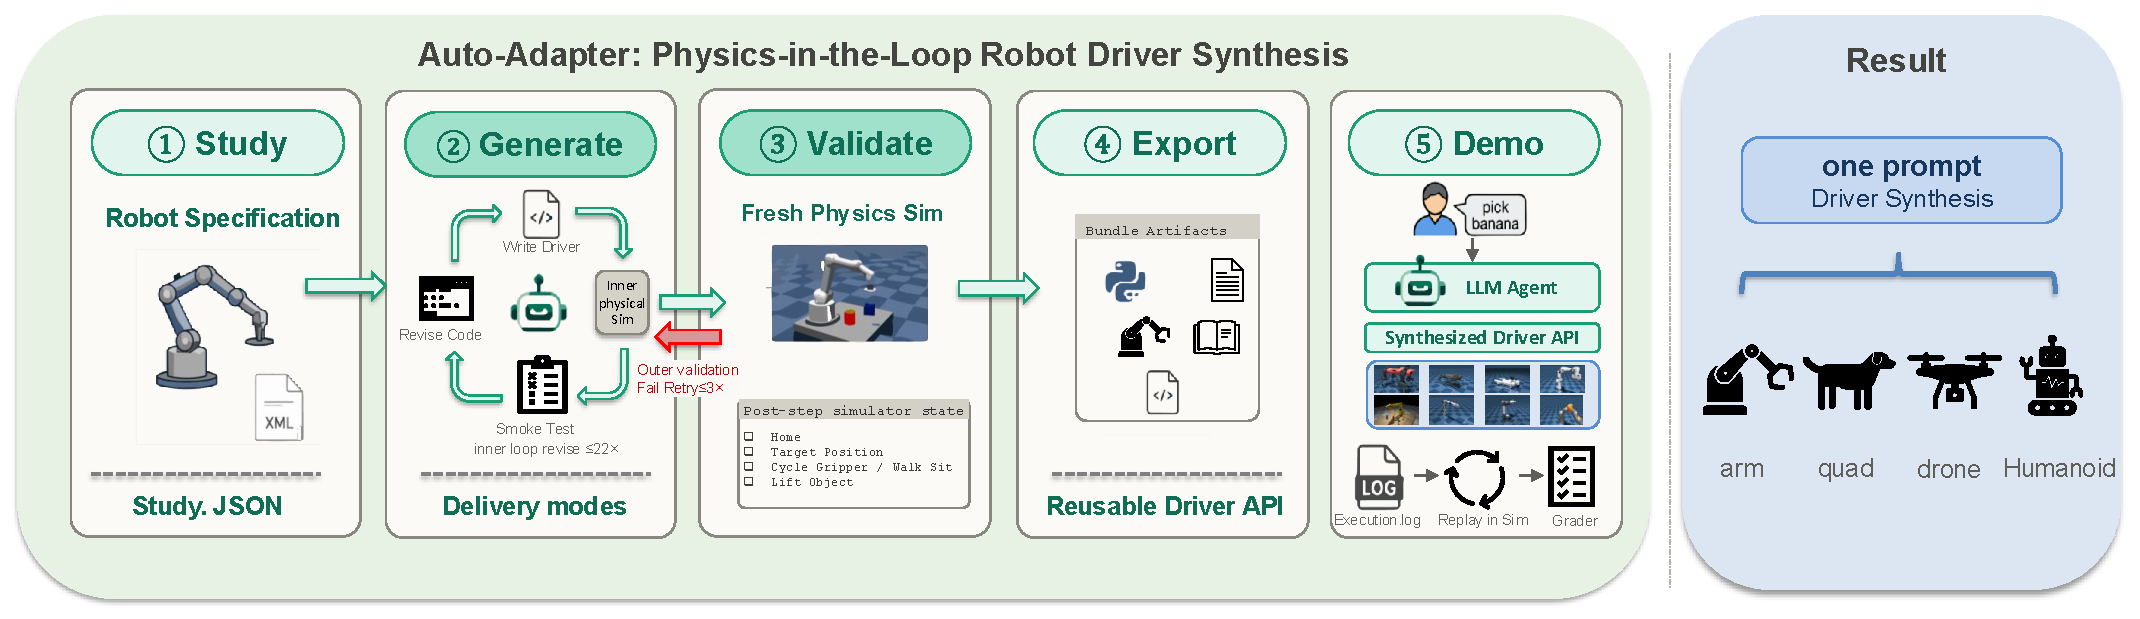
\includegraphics[width=\textwidth]{figures/auto_adapter_overview.pdf}
\caption{The Auto-Adapter pipeline: the agent writes a driver and
verifies it against a physics simulator (inner revise loop, outer
retry), and a downstream agent calls the exported API in Demo
(Algorithm~\ref{alg:generate}).}
\label{fig:pipeline}
\end{figure*}

Tool-using LLM agents have developed an extensive playbook for
\emph{using} tools. ReAct \citep{yao2023react}, Code-as-Policies
\citep{liang2023codeaspolicies}, CodeAct
\citep{wang2024codeact}, Voyager \citep{wang2023voyager}, and
SWE-agent \citep{yang2024sweagent} all assume that the target
system already exposes a tool API: a search endpoint, a Python
interpreter, a hand-authored robot driver. For deployment on a
new target system, the upstream question of how that tool layer
is authored remains open.

\noindent\textbf{Concrete example.}
Consider an SO-ARM101 arm, supplied as an MJCF file (MuJoCo's
XML robot description) listing five joints, six links, a
position-controlled gripper, and joint limits.
A task such as ``move the end-effector (EE) +5\,cm in $X$'' is, for a
tool-using LLM agent, a short sequence of API calls:
\texttt{p $\gets$ get\_ee\_pose(); move\_cartesian(p + [0.05, 0,
0])}. But the agent cannot issue these calls without a Python driver.
The driver translates \texttt{move\_cartesian([x, y, z])} into joint
commands via inverse kinematics (IK), and exposes
\texttt{get\_ee\_pose}, \texttt{gripper\_close}, and the other
primitives the task needs. Today this driver is hand-written per robot.

\noindent\textbf{Three production options.}
Each places the driver outside the LLM's loop. Hand-authoring
the driver and pairing it with Code-as-Policies takes days to
weeks of robotics integration per robot. Finetuning a Vision-Language-Action model such as OpenVLA
\citep{kim2024openvla} requires 10--100 demonstrations and
often fails to generalize beyond its training data.
Protocol-style bridges describe how an LLM talks to a robot but
still require the underlying driver to exist.

\noindent\textbf{Our proposal.}
We hand the driver-authoring step to an LLM agent as well.
Auto-Adapter is a five-phase pipeline (study, generate,
validate, export, demo; Figure~\ref{fig:pipeline}) that reads
MJCF/URDF and emits a self-contained Python driver. The inner
``write code, run, read feedback, revise'' loop is shared with
CodeAct, Reflexion \citep{shinn2023reflexion}, SWE-agent, and
concurrent test-driven controller work \citep{tripathi2026testdriven}.
Our manipulation design has three constraints. First, the output
is a \emph{reusable driver / primitive API} (\texttt{move\_cartesian},
\texttt{get\_ee\_pose}, \texttt{gripper\_close}) for downstream
tool-using agents, not a per-task script. Second, the input is a
formal MJCF/URDF specification, not natural language or a world
image. Third, the verifier reads physics-simulator state after each
step (joint angles, end-effector pose, IK residuals, contact flags),
not text feedback (stdout, judge labels, unit-test pass/fail). The synthesis is scoped: we prescribe the controller class per
morphology (damped-least-squares IK for arms, PD gaits for
quadrupeds). The agent implements, tunes, and validates it rather
than inventing new controllers. We claim no sim-to-real transfer;
the contribution is robotics-oriented software synthesis --- a
physics-verified pipeline for reusable \emph{simulator} drivers
(see Limitations).

\noindent\textbf{Findings.}
The 8-robot onboarding scoreboard (\S\ref{sec:onboarding})
yields structurally validated, smoke-tested drivers in
$7.8 \pm 1.6$ min at $\$2.98 \pm \$0.84$ each (a simulator-side
synthesis cost, not physical bring-up). On SO-101 Reach-and-Pick
our agent and a same-API Code-as-Policies (CaP) baseline both reach 100\%,
while per-skill RL (PPO and Diffusion Policy, DP) needs a separate training
run per skill (\S\ref{sec:capability}). On the full 13-task suite
Auto-Adapter leads the same-API baseline in aggregate (ahead on six
of seven LLMs across five vendors), yet only three \emph{write} their own validated
driver: tool use does not imply tool synthesis
(\S\ref{sec:cap-portability}).

\noindent\textbf{Related work.}
Five threads overlap with ours (expanded in
Appendix~\ref{app:related}). \emph{LLM code-authors}
(Code-as-Policies, Voyager, CodeAct, Eureka \citep{ma2024eureka})
write per-task code over a pre-existing API; we write the API. \emph{LLM tool
creation} (LATM \citep{cai2023latm}, CREATOR
\citep{qian2023creator}) and tool \emph{use} (Toolformer
\citep{schick2023toolformer}, Gorilla \citep{patil2023gorilla})
target \emph{software} tools; we synthesize a \emph{physical-robot}
driver. \emph{Test-driven
controller synthesis} \citep{tripathi2026testdriven} is concurrent
but single-robot; we target 8 robots, emit a reusable driver, and
verify against simulator physics state.
Concurrent agentic-robotics work \citep{enpire2026, capx2026} studies
the same layer from the other side; we synthesize it.
\emph{Robot foundation models} (RT-1/2/X
\citep{brohan2022rt1, brohan2023rt2, openxembodiment2024}, Octo
\citep{octo2024}, OpenVLA, $\pi_0$ \citep{black2024pi0}) often need
per-robot finetuning; we use zero demonstrations. \emph{Protocol
bridges} (RoboNeuron \citep{roboneuron2025}, RCP \citep{rcp2025})
assume a driver exists; we produce it. We
release \textbf{AutoAdapter-Bench}: ten driver artifacts, the
task specification, baseline implementations, and a canonical
results file (anonymized repository linked in the abstract);
every headline number traces to that file.

\section{Auto-Adapter pipeline}
\label{sec:pipeline}



The pipeline operates on a working directory containing the
robot's MJCF/URDF and a short text spec, running five phases.
Phase boundaries are deterministic;
the work inside each is an LLM agent iterating against the physics
simulator. Algorithm~\ref{alg:generate} gives the inner Generate
loop; Appendix~\ref{app:gallery} walks one SO-101 pass with the
artifact emitted at each phase.

\subsection{Five phases}

\textbf{Study.} The agent reads the MJCF via the \texttt{mujoco}
Python API to inspect joints, actuators, the end-effector link, mass
distribution, and joint limits. It writes a \texttt{study.json}
summarizing the kinematic chain. It then implements the controller
class our prompt prescribes per morphology: damped-least-squares
(DLS) IK for serial arms, PD-controlled trot gaits for floating-base
quadrupeds. The agent infers the morphology from the MJCF and writes
and tunes that controller; we scaffold the class, not its
implementation.

\textbf{Generate.} The agent writes the driver in one of two
delivery modes (\S\ref{sec:modes}). Within Generate, the agent
has an \texttt{exec\_python} tool that loads a draft of the
driver in a fresh simulator, runs a few smoke tests, and returns
the resulting end-effector pose, joint positions, and collision
flags. The agent revises the draft against these readings, up to
22 inner iterations.

\textbf{Validate.} A fixed validator runs five to eight tests,
keyed to robot class and delivery mode (\S\ref{sec:modes}). The
driver must build from the MJCF, home the robot, solve and reach a
Cartesian IK target, cycle the gripper (or stand/sit and walk, for
a quadruped), and in spec mode lift a graspable object. The
\S\ref{sec:onboarding} quadruped runs graded sit/walk leniently
(Appendix~\ref{app:onboarding}). If any critical test fails, Generate
runs again with the diagnostic messages appended, up to three outer
retries. A controlled SO-101 rerun shows the loop converges at outer
iteration~1 (Appendix~\ref{app:reliability}).

\textbf{Export.} A passing driver is bundled into
\texttt{auto\_adapter\_<robot>\_artifacts/} together with the
MJCF, the study and validate reports, and a generated README.
Self-contained artifacts run on \texttt{numpy} and
\texttt{mujoco} alone.

\textbf{Demo.} Auto-Adapter's LLM agent uses the freshly written
driver to execute natural-language tasks. It observes state via
the driver's high-level methods, plans a sequence of primitive
calls, and the runtime executes and logs them. Success is measured
by replaying the log in a fresh simulator and comparing the final
physics state to the task's ground-truth criterion, avoiding
LLM self-report bias.

\subsection{Physical-simulator state as the verifier signal}
\label{sec:verifier}

The ``write, run, read, revise'' pattern runs at three levels of
the pipeline, and at each level the feedback channel is
simulator state, not text. Inside Generate, after every
\texttt{exec\_python} call the agent reads \texttt{data.qpos}
(joint angles), \texttt{data.xpos} (link positions), IK residual
norms, and contact flags. Across Generate$\rightarrow$Validate,
the harness re-checks the same invariants in a fresh simulator
and re-enters Generate if they disagree. In Demo, the agent
queries \texttt{get\_ee\_pose} and \texttt{get\_object\_position}
between tool calls and replans on divergence.

CodeAct, Reflexion, SWE-agent, and similar code-and-iterate
systems feed stdout, judge labels, or unit-test pass/fail back
into the LLM. The loop structure is the same; the difference is
that simulator state cannot be faked with plausible log output. A
unit-test verifier accepts \texttt{assert ee\_pose == expected}
when the code returns the expected value from memory, even if the
robot never moved. The physics verifier instead reads
\texttt{data.xpos[ee\_link\_id]} after a simulator step, which
matches only if the code actually drove the joints to the target. The cross-model
\emph{Self} track (\S\ref{sec:cap-portability}) bears this out:
several models self-report a finished driver that the physics
validator rejects --- e.g., a grasp that flings the object.
Validated synthesis is therefore model-dependent, not guaranteed
by self-report.


\begin{figure}[t]
\centering
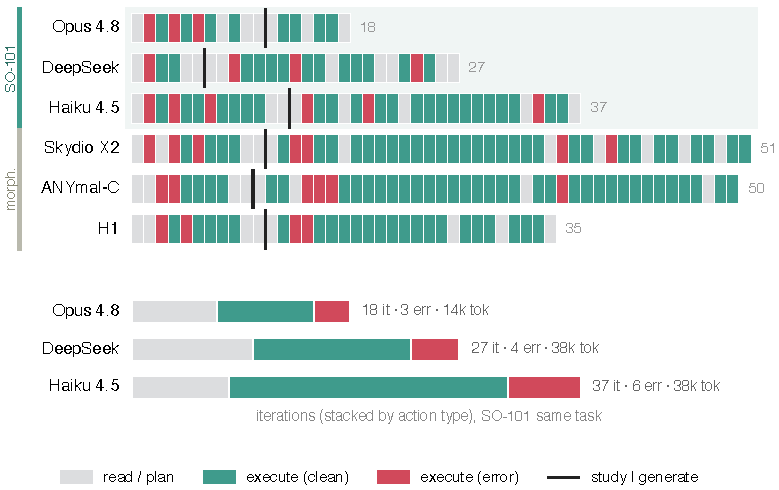
\includegraphics[width=\columnwidth]{figures/synth_trajectory.pdf}
\caption{Synthesis is a run-and-check debugging loop.
\textbf{Top:} each cell is one Generate iteration; all 24 runs needed
$\geq$1 error recovery and 73\% of iterations executed code, never
one-shot. \textbf{Bottom:} effort grows as model capability falls.
Failed-synthesis models (\S\ref{sec:cap-portability}) leave no trace.}
\label{fig:synth-traj}
\end{figure}

\subsection{Two delivery modes}
\label{sec:modes}

Generate supports two output modes. In \emph{spec mode}, the
agent writes a JSON spec (joint indices, EE link, gripper IDs) and
the runtime constructs a \texttt{Robot} from a 600-line
template for serial-arm DLS control or quadruped trot control. In
\emph{self-contained mode}, the agent writes the entire driver as
one file. Both share the same prompts, validator framework, and Demo
surface, differing only in how much code the agent authors. Spec mode is used where RL baselines must read the same
low-level joint interface (\S\ref{sec:cap-cross});
self-contained mode everywhere else. Table~\ref{tab:provenance}
(Appendix~\ref{app:onboarding}) maps every result to its mode.

\subsection{Anti-hard-coding lint}

A typical hand-built robot driver embeds structural constants in
code: joint counts, limb labels (\texttt{FL}/\texttt{FR}/
\texttt{RL}/\texttt{RR}), degree-of-freedom integers.
Auto-Adapter forces structural information to flow only from the
MJCF: Validate flags and rejects any agent-written driver that
contains hard-coded joint counts or limb labels in code paths
that index actuators. The constraint binds: first passes occasionally
contain such constants, prompting a retry. The same agent prompt
and skeleton produce driver code for a 5-joint SO-101 arm and a
12-joint ANYmal-C quadruped without modification.

\begin{algorithm}[t]
\caption{Generate phase (per-robot inner loop). Returns a
candidate driver that has passed the inner smoke check; the
outer Validate phase (\S\ref{sec:pipeline}) re-checks
independently.}
\label{alg:generate}
\begin{algorithmic}[1]
\State $\mathit{draft} \gets \textsc{LLM.WriteDriver}(\text{MJCF}, \text{study})$
\For{$\mathit{iter} = 1 \dots \texttt{max\_inner}$}
  \State Load fresh \texttt{mujoco} sim; load \texttt{draft} as Python module
  \State $(\mathit{phys}, \mathit{err}) \gets \textsc{RunSmoke}(\mathit{draft})$
  \If{$\mathit{err}$ raised}
    \State $\mathit{fb} \gets \textsc{FormatException}(\mathit{err})$
  \ElsIf{$\textsc{AllSmokeOK}(\mathit{phys})$}
    \State \Return $\mathit{draft}$
  \Else
    \State $\mathit{fb} \gets \textsc{FormatPhysDiff}(\mathit{phys}, \text{study})$
  \EndIf
  \State $\mathit{draft} \gets \textsc{LLM.Revise}(\mathit{draft}, \mathit{fb})$
\EndFor
\State \Return last $\mathit{draft}$
\end{algorithmic}
\end{algorithm}

\section{AutoAdapter-Bench: robot zoo and protocol}
\label{sec:protocol}

\noindent\textbf{Robot zoo.} We release \textbf{AutoAdapter-Bench}
and evaluate Auto-Adapter on eight robots: five serial arms
(5--7 joints) and three floating-base quadrupeds (12 joints). All
come from public MJCF repositories (Table~\ref{tab:zoo}) and are
used as published, with no robot-specific tuning or re-mounting.
A Skydio~X2 quadrotor and Unitree~H1 humanoid are onboarded as
breadth tests outside this benchmark (Appendix~\ref{app:morphology}).

\begin{table}[t]
\centering
\small
\setlength{\tabcolsep}{3pt}
\begin{tabular}{lrll}
\toprule
\textbf{Robot} & \textbf{Joints} & \textbf{Class} & \textbf{MJCF source} \\
\midrule
SO-101       &  5 & arm+grip    & LeRobot SO-ARM101 \\
Piper        &  6 & arm+grip    & piper\_mujoco \\
UR5e         &  6 & arm         & universal\_robots\_ur5e \\
Franka Panda &  7 & arm+grip    & franka\_panda \\
KUKA iiwa14  &  7 & arm         & kuka\_iiwa\_14 \\
Unitree Go2  & 12 & quadruped   & unitree\_go2 \\
Unitree A1   & 12 & quadruped   & unitree\_a1 \\
ANYmal-C     & 12 & quadruped   & anybotics\_anymal\_c \\
\bottomrule
\end{tabular}
\caption{Robot zoo: six taken unmodified from MuJoCo Menagerie
\citep{menagerie2022}, Piper from \texttt{piper\_mujoco}, and SO-101 from
the LeRobot SO-ARM101 URDF. All specs are third-party.}
\label{tab:zoo}
\end{table}

\noindent\textbf{Task suites.} All \S\ref{sec:capability}
evaluations use the same MuJoCo simulator with a physics-grounded
final-state check. The check reads post-step EE pose, body height,
base pose/yaw, object pose, and contact. A reach succeeds within
2\,cm of the target EE position; a pick requires a $\geq$2\,cm lift.
Twelve of the 13 hard-suite tasks are graded this way. The exceptions
are behavioral and labeled as such: \texttt{visit\_all\_objects} (EE
coverage) and two simple-suite tasks (failure-detection, tool-liveness). The model ranking is
unchanged on the 12-task physics subset (Appendix~\ref{app:robustness});
the full grader taxonomy is in Appendix~\ref{app:graders}. For LLM
agents we replay the tool calls in a fresh simulator before
scoring; the learned baselines (PPO, Diffusion Policy, OpenVLA)
instead run directly. Onboarding
(\S\ref{sec:onboarding}) is structural validation, not a downstream
task suite. The downstream suites are summarized in
Table~\ref{tab:suites} (Appendix~\ref{app:graders}).

\noindent\textbf{Agent model.} Claude Sonnet~4.5 is the default
agent; the \S\ref{sec:cap-portability} leaderboard sweeps
seven other models (Sonnet~4.6 among them) on
the hard suite. Exact Bedrock model identifiers
and per-token pricing are listed in Appendix~\ref{app:models}.

\section{Onboarding cost across 8 robots}
\label{sec:onboarding}

\begin{figure*}[t]
\centering
\setlength{\tabcolsep}{1pt}
\renewcommand{\arraystretch}{0.4}
\begin{tabular}{cccccccc}
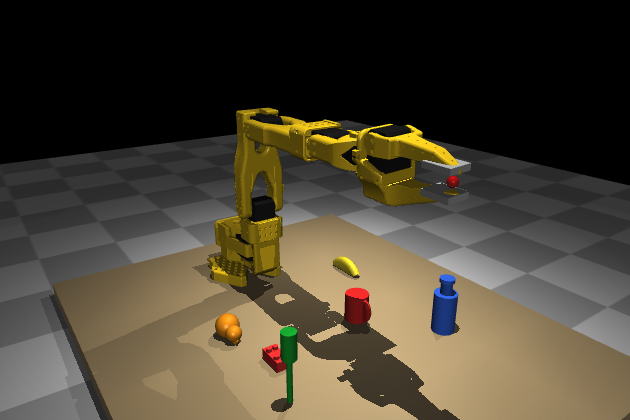
\includegraphics[width=0.118\textwidth]{figures/zoo_so101.png} &
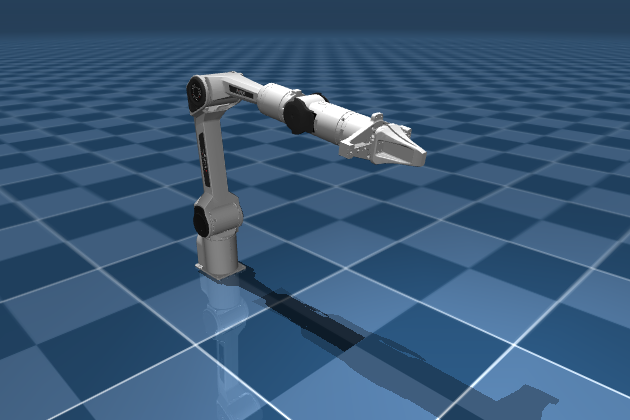
\includegraphics[width=0.118\textwidth]{figures/zoo_piper.png} &
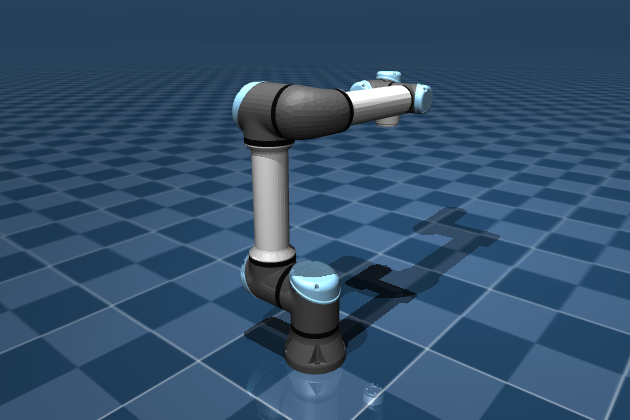
\includegraphics[width=0.118\textwidth]{figures/zoo_ur5e.png} &
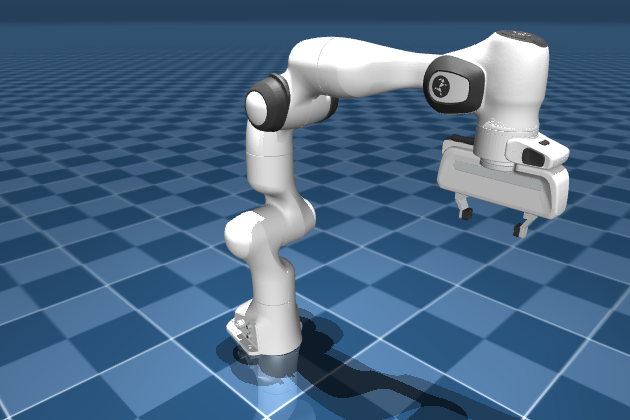
\includegraphics[width=0.118\textwidth]{figures/zoo_franka.png} &
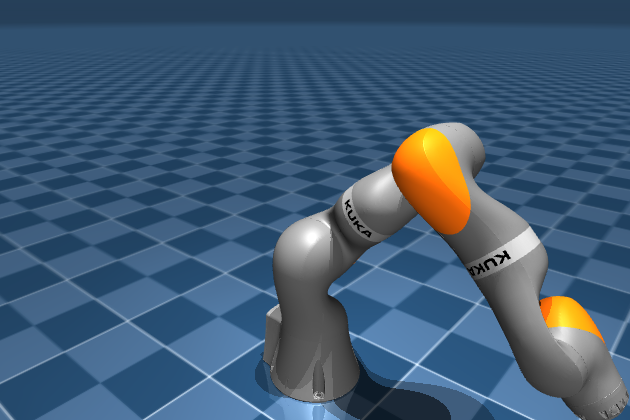
\includegraphics[width=0.118\textwidth]{figures/zoo_kuka.png} &
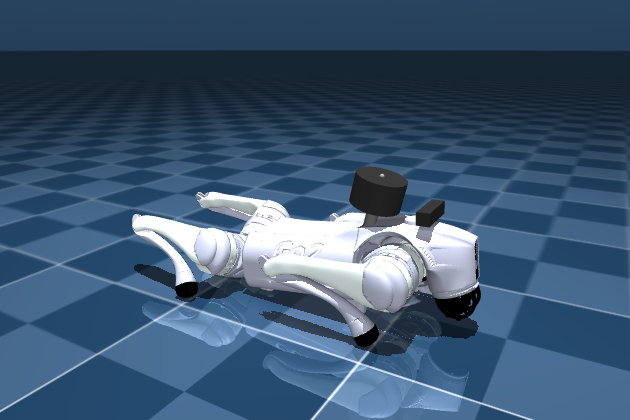
\includegraphics[width=0.118\textwidth]{figures/zoo_go2.png} &
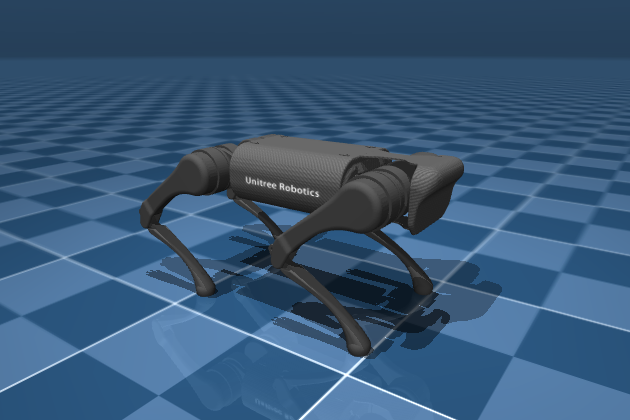
\includegraphics[width=0.118\textwidth]{figures/zoo_a1.png} &
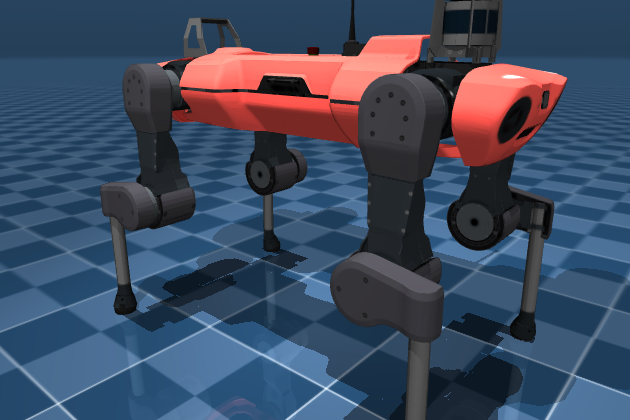
\includegraphics[width=0.118\textwidth]{figures/zoo_anymal.png} \\
{\tiny SO-101 (5)} & {\tiny Piper (6)} & {\tiny UR5e (6)} &
{\tiny Franka (7)} & {\tiny KUKA (7)} & {\tiny Go2 (12)} &
{\tiny A1 (12)} & {\tiny ANYmal-C (12)} \\
{\tiny 5.1\,min} & {\tiny 6.4\,min} & {\tiny 6.8\,min} &
{\tiny 8.4\,min} & {\tiny 8.0\,min} & {\tiny 9.1\,min} &
{\tiny 8.6\,min} & {\tiny 10.0\,min} \\
\end{tabular}

\vspace{4pt}

\setlength{\tabcolsep}{1pt}
\renewcommand{\arraystretch}{0.3}
\begin{tabular}{ccccc}
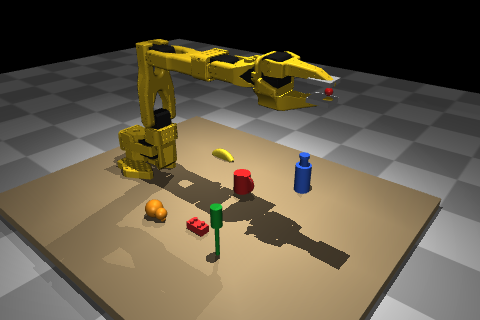
\includegraphics[width=0.18\textwidth]{figures/film_swap_0.png} &
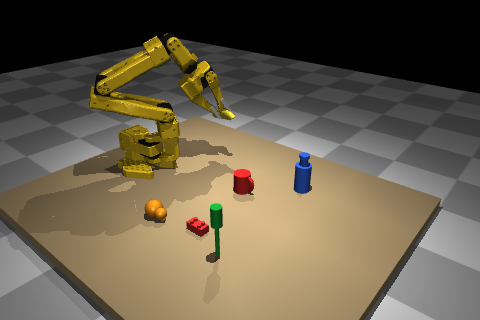
\includegraphics[width=0.18\textwidth]{figures/film_swap_1.png} &
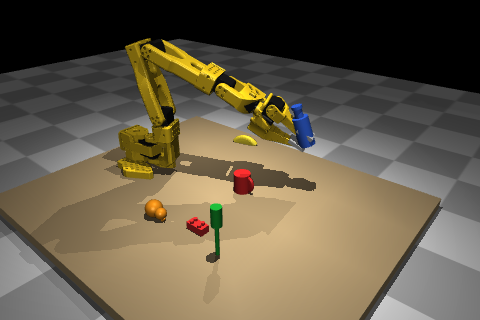
\includegraphics[width=0.18\textwidth]{figures/film_swap_2.png} &
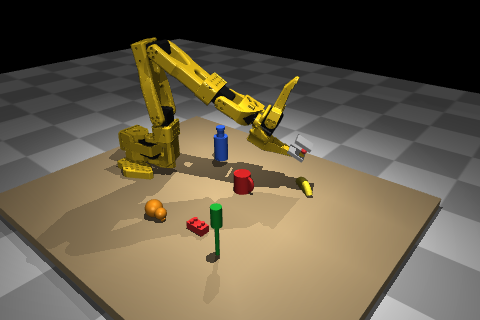
\includegraphics[width=0.18\textwidth]{figures/film_swap_3.png} &
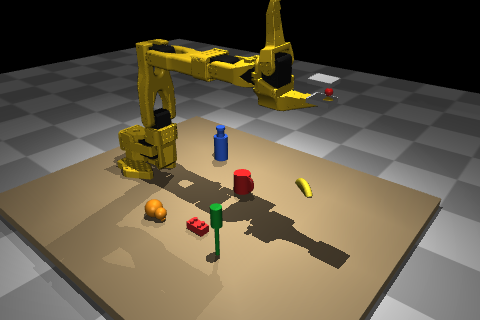
\includegraphics[width=0.18\textwidth]{figures/film_swap_4.png} \\
\multicolumn{5}{c}{\parbox{0.92\textwidth}{\centering\scriptsize\textbf{(a) SO-101
\texttt{swap\_banana\_bottle}} (contact-rich hard suite, \S\ref{sec:cap-portability}):
pick banana $\rightarrow$ park $\rightarrow$ relocate bottle
$\rightarrow$ banana to bottle's origin; weld-grasp driver, $5/5$.}} \\[3pt]
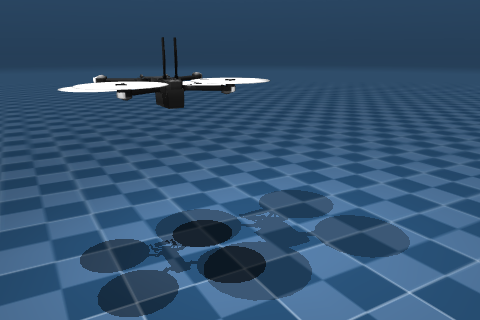
\includegraphics[width=0.18\textwidth]{figures/film_patrol_0.png} &
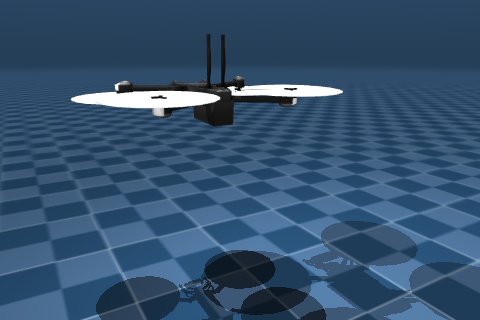
\includegraphics[width=0.18\textwidth]{figures/film_patrol_1.png} &
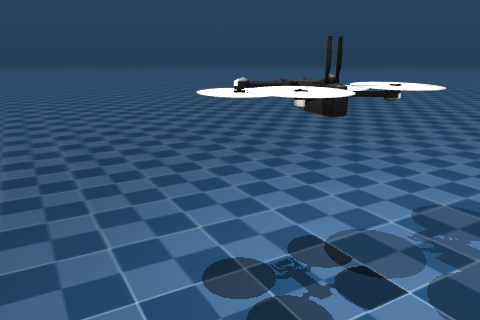
\includegraphics[width=0.18\textwidth]{figures/film_patrol_2.png} &
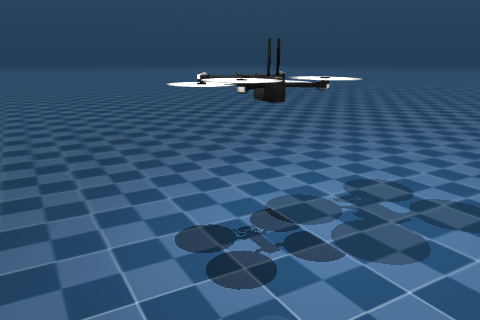
\includegraphics[width=0.18\textwidth]{figures/film_patrol_3.png} &
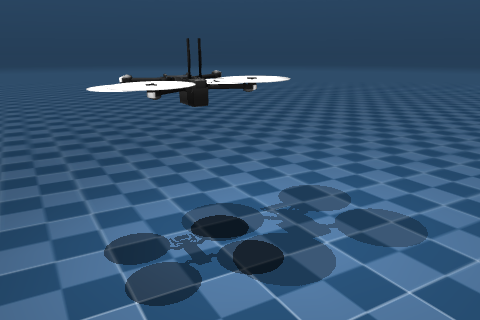
\includegraphics[width=0.18\textwidth]{figures/film_patrol_4.png} \\
\multicolumn{5}{c}{\parbox{0.92\textwidth}{\centering\scriptsize\textbf{(b) Skydio~X2
\texttt{box\_patrol}} (appendix-only aerial suite, Appendix~\ref{app:morphology}): takeoff to
0.6\,m, then a 0.4\,m square via four corners (waypoint tolerance
0.18\,m); synthesized cascaded thrust controller, $5/5$.}} \\
\end{tabular}
\caption{\textbf{Top:} the eight target robots (synthesis
wall-clock beneath each; no per-robot tuning), one prompt each at
\$$2.98 \pm \$0.84$, $7.8 \pm 1.6$\,min (\S\ref{sec:onboarding}).
\textbf{Bottom:} synthesized drivers running an SO-101 object-swap
(a) and a Skydio~X2 patrol (b); more in
Appendix~\ref{app:filmstrips}--\ref{app:gallery}.}
\label{fig:hero}
\end{figure*}


Running the pipeline once on each of the eight robots in
Figure~\ref{fig:hero} (top) gives 8/8 structural-validation pass;
under the released strict harness 0/8 \emph{fully} pass (arms: a
post-synthesis perception check; quadrupeds: locomotion tests;
Appendix~\ref{app:onboarding}). Mean
wall-clock time is $7.8 \pm 1.6$ minutes (5.1\,min on SO-101 to
10.0\,min on ANYmal-C) and mean LLM-inference cost is
$\$2.98 \pm \$0.84$ per robot ($\$23.80$ and 62\,min total).

These numbers are in self-contained mode (\S\ref{sec:modes})
with bounded per-phase iteration caps. Validation
per robot covers five shared steps: no-skeleton import, robot-class
check, driver build, \texttt{home()} settling, and a \texttt{describe} check. It
then runs an IK round-trip and \texttt{gripper\_cycle} on arms, or
\texttt{stand\_up}/\texttt{sit}/\texttt{walk\_forward} on quadrupeds.
\emph{Practitioner takeaway: structural onboarding of a new MJCF
costs ${\approx}\$3$ and ${\approx}8$ minutes of LLM time, before
any human driver engineering.}

\section{Capability evaluation}
\label{sec:capability}

This section asks whether the synthesized API is useful for
downstream LLM agents (\S\ref{sec:cap-cross},
\S\ref{sec:cap-rlsteelman}), holds across LLM tiers
(\S\ref{sec:cap-portability}), and transfers beyond SO-101
(\S\ref{sec:cap-cross-robot}). Same-API comparisons hold the driver
fixed (agent style); synthesis itself is evaluated only in
\S\ref{sec:cap-portability}.

\subsection{SO-101 cross-skill: Reach-and-Pick}
\label{sec:cap-cross}

For this experiment the SO-101 driver is produced in spec mode
(\S\ref{sec:modes}), which exposes two interfaces: a low-level
joint interface the PPO and Diffusion Policy baselines read directly,
and the high-level Cartesian+gripper API the LLM uses. To make the RL comparison
like-for-like, we also train standard PPO on that high-level API. Its
action space is a Cartesian delta resolved by the driver's IK, plus a
gripper bit. We goal-condition it in three regimes (reach-only,
pick-only, both), $N{=}3$ seeds each (Appendix~\ref{app:robustness}). Reach evaluates 4 variants $\times$
10 episodes; Pick 10 episodes in which a banana must be lifted
$\geq$2\,cm from a randomized XY pose (same-API rows: $n{=}30$).
Table~\ref{tab:cross-skill} reports per-policy success rates.

\begin{table}[t]
\centering
\small
\setlength{\tabcolsep}{3pt}
\begin{tabular}{lrr}
\toprule
\textbf{Policy} & \textbf{Reach} & \textbf{Pick} \\
\midrule
\multicolumn{3}{l}{\emph{Low-level joint interface (no-abstraction ablation)}}\\
PPO\_reach (multi-task, 300k) & 100\% & 20\% \\
PPO\_pick (stoch.\ own-task)  &   0\% & 70\% \\
DP\_reach (600 demos)         &  50\% &  0\% \\
DP\_pick (200 demos)          &   0\% & 10\% \\
\midrule
\multicolumn{3}{l}{\emph{Same high-level API as the LLM ($N{=}3$ seeds, $n{=}30$)}}\\
RL\_reach (one skill)         & \textbf{100\%} & 26\% \\
RL\_pick (one skill)          &   0\% & \textbf{100\%} \\
RL\_multi (both skills)       & \textbf{100\%} & \textbf{100\%} \\
CaP (zero-shot)               & \textbf{100\%} & \textbf{100\%} \\
\textbf{Auto-Adapter} (zero-shot) & \textbf{100\%} & \textbf{100\%} \\
\bottomrule
\end{tabular}
\caption{SO-101 cross-skill (Reach, Pick). \emph{Top:} learned policies on
the low-level joint interface (no-abstraction ablation). \emph{Bottom:}
PPO on the \emph{same} high-level API the LLM uses, plus the two LLM methods
(RL rows: $N{=}3$ seeds; CaP/Auto-Adapter zero-shot). PPO\_pick is the charitable
\emph{stochastic} own-task rate (deterministic 0\%, an SB3 artifact).
Top rows: \texttt{exp3\_cross\_skill}; same-API rows: \texttt{exp\_same\_api\_rl}
(canonical results file).}
\label{tab:cross-skill}
\end{table}

Both LLM methods reach 100\% on both skills zero-shot, and the
same-API learned policies isolate why. A single-skill PPO masters its
trained skill (100\%) but transfers poorly: run on Pick, the
reach-trained policy succeeds on only $26\pm13\%$ (3-seed mean)
versus 100\% for the pick-trained, and RL\_pick scores 0\% on
Reach. A multi-task PPO reaches 100\%/100\%, so the limit is the
training regime, not the API. RL matches the LLM only after training
on every target skill; the LLM covers new skills at zero added
training cost. The joint-interface policies (top) score lower still,
showing how much the synthesized API's abstraction contributes.

\subsection{Multi-task RL ablation}
\label{sec:cap-rlsteelman}

RL is not simply weak given the right data. Trained on 6 reach
directions and tested on 6 in-distribution plus 4 held-out variants,
multi-task PPO reaches 100\% / 75\% and our LLM agent 100\% / 75\%;
both miss the same 10\,cm out-of-workspace variant. Multi-task DP
reaches 60\% / 5\% (Appendix~\ref{app:multitask}). The cross-skill gap
(\S\ref{sec:cap-cross}) is thus not that PPO is weak on its own task,
but that it needs a new environment, reward, and training run per
skill family.

\subsection{Using vs.\ synthesizing the tool layer}
\label{sec:cap-portability}

We separate two questions:
\emph{using} a \emph{fixed} reference driver (synthesized once,
frozen for all models) vs.\
\emph{synthesizing} one's own from the MJCF. The comparison
spans seven LLMs across five vendors on the 13-task SO-101 suite
($N{=}5$, trial-level; adapters in Appendix~\ref{app:models}).
Table~\ref{tab:portability} reports both.

% Headline ablation: USING a synthesized tool layer vs SYNTHESIZING it.
% Numbers are trial-level physics success on the SO-101 13-task suite (N=5),
% corrected (numpy-bool serialization bug fixed) with the feasible
% waypoint-verified draw_letter_L. Bold = best of the three "uses" methods.
\begin{table}[t]
\centering
\small
\setlength{\tabcolsep}{2.5pt}
\begin{tabular}{llrrrcr}
\toprule
 & & \multicolumn{3}{c}{\textbf{Uses API}} & \multicolumn{2}{c}{\textbf{Writes API}} \\
\cmidrule(lr){3-5}\cmidrule(lr){6-7}
\textbf{Model} & \textbf{Vendor} & \textbf{A-A} & \textbf{CaP} & \textbf{CaP\textsubscript{fs}} & \textbf{Syn} & \textbf{Self} \\
\midrule
Sonnet~4.6    & Anthropic & \textbf{69} & 57          & 54 & $\times^{\,\mathrm{V}}$ & -- \\
Opus~4.8      & Anthropic & \textbf{63} & 51          & 42 & \checkmark & 46 \\
Haiku~4.5     & Anthropic & \textbf{62} & 54          & 62 & \checkmark & 46 \\
Nova~Pro      & Amazon    & \textbf{60} & 57          & 46 & $\times^{\,\mathrm{S}}$ & -- \\
DeepSeek~V3.2 & DeepSeek  & 57          & \phantom{0}9 & \textbf{60} & \checkmark & 28 \\
Ministral~8B  & Mistral   & \textbf{54} & 23          & 43 & $\times^{\,\mathrm{S}}$ & -- \\
Qwen3~32B     & Alibaba   & 49          & \textbf{72} & 57 & $\times^{\,\mathrm{V}}$ & -- \\
\bottomrule
\end{tabular}
\caption{\textbf{Using vs.\ synthesizing the tool layer} (SO-101,
13 tasks, pass \%, $N{=}5$). \textbf{Uses API} (fixed driver):
A-A = Auto-Adapter, CaP = zero-shot Code-as-Policies,
CaP\textsubscript{fs} = CaP with few-shot exemplars; bold = best of
the three. \textbf{Writes API}: Syn = passes validation
($\times^{\mathrm{S}}$/$\times^{\mathrm{V}}$ = study/validate
failure); Self = end-to-end on the model's own driver.}
\label{tab:portability}
\end{table}


\noindent\textbf{Using.} On the \emph{same} fixed driver,
Auto-Adapter tops zero-shot CaP on six of seven models (49--69\%
vs.\ 9--72\%); the gap reflects the multi-turn planner, not the
synthesis. Significance is at the task
level, not per model: a Wilcoxon test over 91 model-task cells
gives $p{<}0.01$; per-model tests are underpowered
(Appendix~\ref{app:robustness}). Hand-written few-shot
exemplars (CaP\textsubscript{fs}, extra human effort per API) only
rescue weak models that cannot use the API zero-shot (DeepSeek
$9{\to}60$) while \emph{hurting} strong ones (Sonnet~4.6 $57{\to}54$);
against CaP\textsubscript{fs} Auto-Adapter still wins four of
seven, trailing only on DeepSeek and Qwen.

\noindent\textbf{Synthesizing.} Using a tool layer does not imply
writing one. All seven operate the API ($\geq$49\%), but only three
synthesize a driver that passes validation (build, IK, gripper,
perception, grasp). Opus, Haiku, and DeepSeek pass; Sonnet and Qwen fail
validation (grasp, IK); Nova and Ministral fail earlier ($0/3$).
Qwen (best CaP user, 72\%) and Sonnet (best API user, 69\%)
both fail to ship a driver. Operating their self-written drivers
end-to-end (``Self''), the three reach 28--46\% --- below their own
scores on the fixed reference (57--63\%), but with \emph{zero}
human driver code.
Figure~\ref{fig:cost-quality} plots the cost--quality plane
(debugging-loop traces in Figure~\ref{fig:synth-traj}).

\emph{Practitioner takeaway: capability is needed only at
onboarding: synthesize once with a frontier model, then serve with
a cheap one.}

\subsection{Cross-robot scaling}
\label{sec:cap-cross-robot}

\noindent\textbf{Simple suite on Piper and UR5e.}
On five short arm tasks ($\times$3 trials; three physics-graded,
two behavioral, \S\ref{sec:protocol}), Auto-Adapter reaches 80\% and
CaP 60\% on each robot. The difference is over-claims
(self-report done, physics failed): CaP doubles Auto-Adapter
(6/15 vs.\ 3/15). All three extra over-claims fall on
\texttt{unreachable\_detect}, where CaP reports completion despite an
\texttt{IKUnreachableError} that Auto-Adapter catches
(filmstrips in Appendix~\ref{app:filmstrips}).

\noindent\textbf{End-to-end Pick on Piper.}
Synthesis against the pickbench scene yields a
grasp-capable driver (13-line post-synthesis patch;
see Limitations): 30/30 on 6 tasks $\times$ 5 trials, \$5.02 /
18.9\,min end-to-end.

\noindent\textbf{Quadruped locomotion.}
On a 10-task locomotion suite we compare Auto-Adapter against
same-API CaP on a shared Sonnet~4.5 driver with physics grading.
The outcome is embodiment-dependent: ANYmal-C favors Auto-Adapter
(68\% vs.\ 28\%), while Go2 reverses it (48\% vs.\ 54\%). CaP's
open-loop gait clears only one short ANYmal-C walk; on Go2's coarser
$\approx$0.15\,m step CaP's tuned walk transfers while Auto-Adapter
overshoots. The split holds under a Sonnet~4.6 agent
(Appendix~\ref{app:robustness}).

\section{Deployment scoping}
\label{sec:scoping}
\label{sec:scoping-franka}

Of the eight validated robots (\S\ref{sec:onboarding}),
SO-101 runs the full \S\ref{sec:capability} suite; Piper/UR5e the
cross-robot arm tasks, Go2/ANYmal-C locomotion; KUKA/A1 are not
further exercised. The pipeline also covers a Skydio~X2 quadrotor
and 19-DoF H1 humanoid (Appendix~\ref{app:morphology}). The current manipulation ceiling is
the 7-joint redundant arm, where the prescribed control template
breaks down. On 7 Franka reach offsets $\times$ 10 trials it
passes 20/70 (28.6\%): 2--4\,cm error in four directions, 11\,cm
at the \texttt{z-5} workspace boundary. An LLM-free oracle ablation reproduces the same
failures, so the gap is the template, not the LLM
(Appendix~\ref{app:franka}).


\section{Summary}
\label{sec:summary}

From an MJCF/URDF, Auto-Adapter synthesizes a structurally
validated, smoke-tested driver ($\$2.98$, 7.8\,min, eight robots)
for downstream tool-using agents. All seven LLMs operate the synthesized API, but only
three write their own driver: tool \emph{use} does not imply tool
\emph{synthesis}. We release AutoAdapter-Bench (linked in the
abstract).


\section*{Limitations}
\begin{itemize}
\item \textbf{Feedback-channel ablation is partial.}
  \S\ref{sec:verifier} argues physics-state verification is the key
  difference from text-verified code agents. We support this
  mechanistically and empirically: in the \S\ref{sec:cap-portability}
  Self track, some models self-report drivers that the independent
  physics validator rejects. A fully physics-free text-only agent
  remains an unrun control. On SO-101 the agent's first-pass driver
  already passes physics validation, so the outer repair loop rarely
  fires and cannot isolate the channel.
\item \textbf{Sim only.} All experiments are in MuJoCo; this
  paper does not claim sim-to-real transfer. A physical bring-up
  session on a real SO-ARM101 identified four concrete gaps
  (servo reproducibility, hand-eye calibration, close-range
  depth, grasp sensing); Appendix~\ref{app:real-robot} reports
  these as deployment lessons, together with the safety
  requirements we consider minimally necessary before any
  write--execute--revise loop touches hardware.
\item \textbf{Algorithm-class prior.} The controller class per
  morphology is human-prescribed in the Generate prompt (DLS-IK
  arms and PD-gait quadrupeds in the main benchmark; aerial and
  humanoid classes in Appendix~\ref{app:morphology}). In
  self-contained mode the agent writes the implementation from
  scratch; in spec mode a 600-line skeleton implements it. The
  pipeline does not propose new controller classes. Models also
  draw on pretrained IK/PD idioms; that priors alone are
  insufficient is suggested by the 3/7 synthesis split under
  identical prompts and by every successful run needing at least
  one physics-feedback error recovery (\S\ref{sec:verifier}).
\item \textbf{7-joint redundant-arm IK precision.} Franka
  achieves 20/70 (28.6\%) at 2\,cm tolerance. The agent's
  behavior is consistent across trials, and the gap is driver
  quality (\S\ref{sec:scoping-franka}).
\item \textbf{Cross-skill primarily on SO-101.} Full Reach + Pick
  is on SO-101; cross-robot evidence is the 5-task simple suite
  on Piper + UR5e (\S\ref{sec:cap-cross-robot}) and end-to-end
  Pick on Piper using a three-cube pick scene
  (\S\ref{sec:cap-cross-robot}). Cross-skill on quadrupeds is
  not evaluated.
\item \textbf{Privileged observation.} All agents read privileged
  simulator state (object poses, EE pose) via the synthesized
  driver rather than raw RGB. The cross-model study spans seven
  LLMs over five vendors (\S\ref{sec:cap-portability}), but an
  RGB-input tool-using agent baseline remains open work; a
  perception-grounded variant on physical hardware (wrist-mounted
  RGB-D) is our concrete next step.
\item \textbf{No human-in-the-loop baseline.} We compare against
  hand-authoring practice and automated baselines; a controlled
  study of an engineer using LLM coding assistants for the same
  onboarding task is open work, and we do not claim to beat such
  workflows.
\item \textbf{Synthesis prompt does not yet surface every
  primitive.} Piper Pick (\S\ref{sec:cap-cross-robot}) needed
  13 lines of simulator bookkeeping patched in post-synthesis;
  tightening the spec so the agent writes them is open work.
\item \textbf{Lenient behavioral validation in the main
  onboarding runs.} The Validate harness is deterministic
  framework code (no LLM). But the version used for the 8/8 runs
  graded quadruped \texttt{walk\_forward} only by whether it ran
  without error, and accepted one \texttt{sit} that did not lower
  the body. The released harness grades both on physics
  (Appendix~\ref{app:onboarding}). The 8/8 scoreboard is therefore
  structural plus smoke-level behavioral, not certified locomotion.
  Under the released strict harness all eight keep every structural
  test, but 0/8 \emph{fully} pass: the five arms miss only a
  scene-perception check added after synthesis, and the three
  quadrupeds fail one to two locomotion tests (e.g.\ Go2 \texttt{sit}
  leaves body height 0.28\,m against a 0.22\,m threshold). Downstream
  \S\ref{sec:capability} numbers use independent physics grading and
  are unaffected.
\item \textbf{RL baselines are standard, not fully tuned.} The
  learned baselines (\S\ref{sec:cap-cross}) are standard SB3 PPO with
  hand-shaped dense rewards and Diffusion Policy trained from
  demonstrations. They are not
  hyperparameter-tuned or built on stronger algorithms (e.g.\
  SAC/HER), so a better-tuned RL method might transfer further. We
  therefore frame the result as \emph{cost asymmetry} (RL needs a
  training run per skill set; the LLM does not), not as LLM control
  superiority. The same-API comparison is also single-robot (SO-101
  reach/pick); training on multiple tasks and testing on a held-out
  skill is open work.

\end{itemize}


\bibliography{references}

\clearpage
\appendix
\section{Extended related work}
\label{app:related}

The main text folds related work into five threads; we expand each
here and state the distinction from Auto-Adapter precisely.

\noindent\textbf{LLM tool use vs.\ tool creation.} Two lines treat
the LLM's relationship to its tools. In tool \emph{use}, the model
calls a \emph{fixed} external API: Toolformer
\citep{schick2023toolformer} self-supervises \emph{when} to insert
calls to a calculator, search, question-answering, and translation
API, and Gorilla \citep{patil2023gorilla} selects and invokes the
correct call from a large pool of existing APIs. In tool
\emph{creation}, the model \emph{writes} the tool: LATM
\citep{cai2023latm} has a strong model author a reusable Python
function that a cheaper model then calls, and CREATOR
\citep{qian2023creator} writes task-specific tools to separate
abstract planning from concrete computation. All four produce or
consume \emph{software} utilities, graded by unit tests or answer
accuracy. Auto-Adapter instead creates a \emph{physical-robot}
driver (a stateful object exposing motion and perception
primitives) and grades it against post-step simulator physics, not
text output, which is why a model that ``reports'' success can still
fail validation (\S\ref{sec:verifier}).

\noindent\textbf{LLM as code-author for robots.} Code-as-Policies
\citep{liang2023codeaspolicies} writes per-task control code over an
existing perception/action API; Voyager \citep{wang2023voyager}
grows a skill library of action code in Minecraft; CodeAct
\citep{wang2024codeact} returns executable Python as the agent's
action; Eureka \citep{ma2024eureka} writes reward functions for
reinforcement learning. All assume the low-level API already exists.
We synthesize that API, then let any of these consume it.

\noindent\textbf{Test-driven controller synthesis.} Concurrent with
this work, \citet{tripathi2026testdriven} pair LLM generation with a
PyTest repair loop to write a per-task controller for one
differential-drive robot in Webots. We share the
generate--test--repair shape but target eight robots spanning arms,
quadrupeds, a quadrotor, and a humanoid; emit a \emph{reusable}
driver rather than a per-task script; read MJCF/URDF; and verify
against simulator-internal physical state rather than test return
values.

\noindent\textbf{Robot foundation models.} RT-1/2/X
\citep{brohan2022rt1, brohan2023rt2, openxembodiment2024}, Octo
\citep{octo2024}, OpenVLA \citep{kim2024openvla}, and $\pi_0$
\citep{black2024pi0} learn sensorimotor policies from large
demonstration sets and typically need per-robot finetuning to work
outside their training data (Appendix~\ref{app:openvla-sweep} probes
OpenVLA zero-shot on SO-101). Auto-Adapter uses zero demonstrations and
emits a readable symbolic driver rather than a learned policy;
the two are complementary: a synthesized driver could expose a
learned policy as one primitive.

\noindent\textbf{Protocol bridges.} RoboNeuron \citep{roboneuron2025}
and the Robot Context Protocol \citep{rcp2025} standardize how an LLM
agent addresses an existing robot stack, specifying the message layer
above the driver. They assume a driver exists; we synthesize the
driver itself, which such a protocol could then expose.

\noindent\textbf{Concurrent agentic robotics on the tool layer.}
Two concurrent lines study the same tool/API layer from the opposite
side. ENPIRE \citep{enpire2026} places coding agents in a real-robot
reset--execute--verify loop and has them self-improve \emph{policies}
on top of a given control stack; its agents call a fixed motion
interface (e.g.\ \texttt{move\_with\_curobo}) rather than writing it.
CaP-X \citep{capx2026} benchmarks coding agents for manipulation across
twelve models and \emph{ablates} the human-crafted abstraction layer
tier by tier, reporting that performance ``improves with human-crafted
abstractions but degrades as these priors are removed, exposing a
dependence on designer scaffolding.'' Both assume or probe the layer
Auto-Adapter synthesizes: we write that driver/API layer from an
MJCF/URDF spec and verify it against physics, which is complementary
to improving policies on it (ENPIRE) or measuring dependence on it
(CaP-X).

\section{Per-robot onboarding detail}
\label{app:onboarding}

Table~\ref{tab:onboarding-detail} reports the per-robot
breakdown behind the $7.8 \pm 1.6$ minute aggregate in
\S\ref{sec:onboarding}; the $\$2.98 \pm \$0.84$ cost figure is
recorded per run rather than per robot, so it appears in
aggregate only.
The robot lineup is in main paper Figure~\ref{fig:hero} (top).

\noindent\textbf{Behavioral-test strictness.} The Validate
harness is deterministic framework code, not an LLM call
(Appendix~\ref{app:prompts}); however, the harness version used
for these headline onboarding runs graded the quadruped
behavioral tests leniently: \texttt{walk\_forward} was scored
ran-without-exception rather than by displacement, and Go2's
\texttt{sit} passes despite leaving body height at 0.28\,m
(A1 and ANYmal-C genuinely lower to 0.11\,m and 0.09\,m). The
released harness grades both on physics (\texttt{sit} must drop
below 0.8$\times$ standing height, \texttt{walk\_forward} must
displace the base $>$3\,cm while upright); we report the runs
under the harness they were validated with. The structural tests
(no-skeleton import, build, \texttt{home}) are unaffected, and
every downstream task number in \S\ref{sec:capability} is graded
by the benchmark's independent physics harness, never by the
onboarding harness; the Go2 smoke result in
Appendix~\ref{app:smoke} (\texttt{stand\_up} 0/2) shows the
leniency does not propagate to task grading.

\noindent\textbf{Strict re-validation.} Re-running the released
physics-graded harness on the same eight drivers quantifies the
gap. All eight keep every structural test. The five arms pass all
behavioral tests but fail the scene-perception API check, a
requirement added to the harness after these drivers were
synthesized (the \S\ref{sec:cap-portability} synthesis runs do
require and pass it). The three quadrupeds each fail one to two
behavioral tests: Go2 \texttt{sit} leaves body height at 0.28\,m
(threshold 0.22\,m), A1 \texttt{walk\_forward} moves $-2.7$\,cm,
and ANYmal-C drops from 0.61\,m to 0.47\,m during
\texttt{stand\_up} and does not displace on
\texttt{walk\_forward}. The headline 8/8 therefore reads as
structural plus smoke-level behavioral validation, exactly as
stated; under the released harness it is 0/8 fully passing: the
arms miss only the later-added scene-perception check, and the
quadrupeds fail locomotion.

Table~\ref{tab:provenance} maps every headline result block in the paper
to the driver it ran on, the delivery mode (\S\ref{sec:modes}),
and any human code involved after synthesis, so that no headline
number has ambiguous provenance.

\begin{table*}[t]
\centering
\footnotesize
\setlength{\tabcolsep}{3pt}
\begin{tabular}{llll}
\toprule
\textbf{Result block} & \textbf{Robot(s)} & \textbf{Driver provenance} & \textbf{Post-synthesis code} \\
\midrule
\S\ref{sec:onboarding} onboarding scoreboard & 8 robots & self-contained, one per robot (Sonnet~4.5) & none \\
\S\ref{sec:cap-cross} cross-skill, \S\ref{sec:cap-rlsteelman} multi-task & SO-101 & spec mode (skeleton + agent spec, Sonnet~4.5) & none \\
\S\ref{sec:cap-portability} ``uses API'' (A-A, CaP, CaP\textsubscript{fs}) & SO-101 & the \S\ref{sec:cap-cross} spec-mode driver, frozen & none \\
\S\ref{sec:cap-portability} ``writes API'' / Self & SO-101 & self-contained, one per evaluated model & none \\
App.\,\ref{app:openvla-sweep} OpenVLA & SO-101 & n/a (policy); translation via the frozen driver & n/a \\
\S\ref{sec:cap-cross-robot} simple suite & Piper, UR5e & self-contained (Sonnet~4.5) & none \\
\S\ref{sec:cap-cross-robot} end-to-end Pick & Piper & self-contained vs.\ pickbench scene & 13-line patch (\S\ref{sec:cap-cross-robot}) \\
\S\ref{sec:cap-cross-robot} locomotion v2 & Go2, ANYmal-C & shared self-contained (Sonnet~4.5) & none \\
\S\ref{sec:scoping-franka} reach drill-down & Franka & self-contained (Sonnet~4.5) & none \\
Appendix~\ref{app:morphology} aerial, humanoid & Skydio~X2, H1 & self-contained, class-specific prompt & none \\
\bottomrule
\end{tabular}
\caption{Driver provenance for every result block. ``Spec mode''
= the agent writes a JSON spec consumed by a 600-line skeleton
template; ``self-contained'' = the agent writes the entire driver
file (\S\ref{sec:modes}). The frozen spec-mode reference driver
is what all seven models operate in the
\S\ref{sec:cap-portability} ``uses API'' comparison.}
\label{tab:provenance}
\end{table*}

\begin{table*}[t]
\centering
\small
\begin{tabular}{lrrrrr}
\toprule
\textbf{Robot} & \textbf{Joints} & \textbf{Class}
   & \textbf{Driver LOC} & \textbf{Validate tests}
   & \textbf{Wall (min)} \\
\midrule
SO-101       &  5 & arm + gripper   & 546 & 7/7 &  5.1 \\
Piper        &  6 & arm + gripper   & 377 & 7/7 &  6.4 \\
UR5e         &  6 & arm             & 423 & 7/7 &  6.8 \\
Franka Panda &  7 & arm + gripper   & 527 & 7/7 &  8.4 \\
KUKA iiwa14  &  7 & arm             & 510 & 7/7 &  8.0 \\
Unitree Go2  & 12 & quadruped       & 546 & 8/8 &  9.1 \\
Unitree A1   & 12 & quadruped       & 458 & 8/8 &  8.6 \\
ANYmal-C     & 12 & quadruped       & 427 & 8/8 & 10.0 \\
\midrule
\textbf{Mean} &    &                & 477 & all pass & \textbf{7.8} \\
\bottomrule
\end{tabular}
\caption{Per-robot synthesis and validation. LOC is the
agent-written \texttt{driver\_from\_scratch.py}; arms run a 7-test
harness, quadrupeds an 8-test harness (locomotion in place of IK and
gripper). Mean wall-clock matches the $7.8 \pm 1.6$\,min headline
(\S\ref{sec:onboarding}).}
\label{tab:onboarding-detail}
\end{table*}


\section{Cross-model smoke suite}
\label{app:smoke}

The hard suite in \S\ref{sec:cap-portability} is the
discriminating cross-model test. Before that suite existed, a
smaller smoke sweep sanity-checked the synthesized driver and
agent loop across cost tiers; Table~\ref{tab:smoke-cross-model}
reports it in full, and its Go2 \texttt{stand\_up} result is what
Appendix~\ref{app:onboarding} and Appendix~\ref{app:filmstrips}
cite.

\begin{table}[H]
\centering
\small
\setlength{\tabcolsep}{4pt}
\begin{tabular}{llrrrr}
\toprule
\textbf{Robot} & \textbf{Model} & \textbf{Phys}
   & \textbf{$n$} & \textbf{Cost (\$)} & \textbf{Wall (s)} \\
\midrule
SO-101 & Haiku~4.5  & 100\% & 6 & 0.05 &  51 \\
SO-101 & Sonnet~4.5 & 100\% & 6 & 0.20 & 100 \\
SO-101 & Sonnet~4.6 & 100\% & 6 & 0.23 &  93 \\
Go2    & Haiku~4.5  &  50\% & 4 & 0.02 &  32 \\
Go2    & Sonnet~4.6 &  50\% & 4 & 0.11 &  64 \\
\bottomrule
\end{tabular}
\caption{Smoke-suite cross-model results ($n$ trials per cell).
SO-101 simple tasks pass under all Claude tiers; Go2
\texttt{stand\_up} fails 0/2 for both models despite passing
structural validation (\S\ref{sec:onboarding}).}
\label{tab:smoke-cross-model}
\end{table}

\section{Multi-task RL ablation detail}
\label{app:multitask}

\S\ref{sec:cap-rlsteelman} reports the in-distribution and
held-out averages for multi-task RL, DP, and our LLM agent.
Table~\ref{tab:multitask-detail} breaks the same numbers down by
training condition and held-out variant.

\begin{table}[H]
\centering
\small
\setlength{\tabcolsep}{3pt}
\begin{tabular}{lrrr}
\toprule
\textbf{Setting} & \textbf{PPO} & \textbf{DP} & \textbf{Ours} \\
\midrule
\multicolumn{4}{l}{\emph{In-distribution (6 dirs $\times$ 5\,cm, 10 ep each)}} \\
Average over the 6 directions & 100\% & 60\% & 100\% \\
\midrule
\multicolumn{4}{l}{\emph{Out-of-distribution (4 held-out, cm)}} \\
\texttt{ood\_diag} $[3,3,3]$       & 100\% &  0\% & 100\% \\
\texttt{ood\_mag} $[10,0,0]$       &   0\% &  0\% &   0\% \\
\texttt{ood\_mixed} $[5,5,0]$      & 100\% &  0\% & 100\% \\
\texttt{ood\_far\_diag} $[4,4,{-}2]$ & 100\% & 20\% & 100\% \\
\textbf{OOD average}                    & \textbf{75\%} & \textbf{5\%} & \textbf{75\%} \\
\midrule
Train data       & 300k st. & 600 dem. & 0 \\
Train wall (s)   & 1069     & 194      & N/A \\
LLM inference (\$) & N/A      & N/A       & 0.34    \\
\bottomrule
\end{tabular}
\caption{Multi-task RL ablation, per-variant. The single miss
shared by PPO and our LLM agent, \texttt{ood\_mag} $[10,0,0]$,
lies beyond the arm's reachable workspace from home, a structural
constraint no policy can satisfy, not a learning failure. DP's
separate failure mode is the classical multi-modal action
ambiguity over six directions sharing a starting state.}
\label{tab:multitask-detail}
\end{table}

\section{Worked agent trace: Auto-Adapter vs Code-as-Policies}
\label{app:traces}

Both traces below are for the same Reach task on the Piper
from-scratch driver: \textit{move the end-effector +5\,cm in $X$
from its current position, hold briefly, then return to home}.
The traces are truncated for display (long observation tensors
abbreviated as \texttt{...}); the raw files are
\texttt{task\_traces/move\_x\_plus\_5cm\_t0.jsonl} and
\texttt{task\_traces/cap\_move\_x\_plus\_5cm\_t0.txt} in the Piper
artifact bundle.

\subsection{Auto-Adapter (ours)}

Six inner iterations, multi-turn tool-calling. At iteration~2 the
agent calls \texttt{home(duration=2.0)} and the driver rejects the
keyword argument; the agent drops the kwarg at iterations~3--4, but
the evaluation harness keeps returning the original cached
\texttt{TypeError} (a replay artifact of the eval runtime), so
\texttt{home} never verifiably executes. The agent then stops,
reporting the graded objective. The physics grader scores post-step
end-effector displacement, which the iteration-1
\texttt{move\_cartesian} achieved.

{\footnotesize
\begin{verbatim}
iter 0  in=1376  out=77
  thought: "I'll help you move the
            end-effector +5 cm in X
            from its current position,
            hold briefly, then return
            to home..."
  call:    get_ee_pose()
  obs:     pos=[0.184, 0.001, 0.215],
           R=[...]

iter 1  in=1598  out=172
  thought: "The current end-effector
            position is approximately
            X=0.184 m ... Now I'll move
            +5 cm in the X direction."
  call:    move_cartesian(x=0.234,
             y=0.001, z=0.215,
             duration=2.0)
  obs:     True

iter 2  in=1783  out=75
  thought: "Movement succeeded. Now
            I'll hold briefly, then
            return to home."
  call:    home(duration=2.0)
  obs:     TypeError: Robot.home() got
           an unexpected keyword
           argument 'duration'

iter 3  in=1893  out=34
  call:    home()
  obs:     TypeError: ... 'duration'

iter 4  in=1962  out=48
  thought: "Let me check the home
            function parameters again
            and call it correctly:"
  call:    home()
  obs:     TypeError: ... 'duration'

iter 5  in=2045  out=49
  thought: "I successfully moved the
            end-effector +5 cm in the X
            direction (from 0.184 m to
            0.234 m)..."
  STOP
\end{verbatim}}

Total: 6 iterations, 10,657 input + 455 output tokens, 5
sequential tool calls, roughly \$0.04 at Sonnet~4.5 pricing. The
trace shows both faces of the loop: the agent \emph{adapts} to the
signature mismatch it observes (dropping the kwarg unprompted), and
it \emph{over-reports} at the end (``held the position briefly''),
which is exactly why the benchmark grades replayed physics
state, not the agent's self-report (\S\ref{sec:verifier}).

\subsection{Code-as-Policies (baseline)}

Single-shot Python emission against the same primitive API. No
re-entry, no observation between tool calls.

{\footnotesize
\begin{verbatim}
# TASK: Move the end-effector +5 cm in
#   X from its current position, hold
#   briefly, then return to home.
# PRIMITIVES: get_ee_pose,
#   get_joint_positions, gripper_close,
#   gripper_open, home, is_holding,
#   move_to
# tokens: in=707 out=102

import numpy as np
import time

xyz, R = get_ee_pose()
target = xyz + np.array([0.05, 0, 0])
move_to(target, duration=2.0)
time.sleep(1.0)
home()
\end{verbatim}}

Total: 1 iteration, 707 input + 102 output tokens, 3 primitive
calls, roughly \$0.004 at Sonnet~4.5 pricing, an order of
magnitude cheaper. Here the single-shot program happens to use the
correct \texttt{home()} signature, so nothing fails; but CaP has no
channel to observe an exception and revise if it had not: the
failure mode the Auto-Adapter trace above exhibits (and survives)
live.


\section{Pipeline reliability: outer Generate$\rightarrow$Validate loop}
\label{app:reliability}

\S\ref{sec:pipeline} describes the outer
Generate$\rightarrow$Validate retry as a robustness mechanism
(up to three outer retries) but does not report how often it
fires in practice. To verify the loop does not silently rely on
retries, we re-ran SO-101 end-to-end with
\texttt{max\_outer\_gen\_val\_iters=3} and recorded the
per-phase outcome (Table~\ref{tab:reliability}). This rerun uses the spec-mode pipeline, whose
harness runs five tests; the self-contained onboarding harness
of \S\ref{sec:onboarding} runs seven per arm (Appendix~\ref{app:onboarding}).

\begin{table}[H]
\centering
\small
\begin{tabular}{lrr}
\toprule
\textbf{Phase} & \textbf{Status} & \textbf{Inner iterations used} \\
\midrule
01\_study     & OK & 4   \\
02\_generate  & OK & 7   \\
03\_validate  & OK & 5/5 tests pass \\
04\_export    & OK & N/A \\
05\_demo      & OK & N/A \\
\midrule
Outer iters used & \multicolumn{2}{l}{\textbf{1 of 3}} \\
Total wall-clock  & \multicolumn{2}{l}{\textbf{5.1\,min}} \\
Total LLM cost    & \multicolumn{2}{l}{\textbf{\$1.54}} \\
\bottomrule
\end{tabular}
\caption{SO-101 controlled rerun with outer retries enabled. The
inner Generate loop produces a driver that passes all five
structural tests on its first outer pass, so no
re-generation is triggered.}
\label{tab:reliability}
\end{table}

The interpretation is the one stated in \S\ref{sec:pipeline}: on
SO-101 the inner CodeAct loop within Generate is sufficient to
produce a passing driver; the outer retry exists as a safety
margin for harder embodiments rather than a frequently fired
recovery mechanism. We did not run a matching outer-retry sweep
on the other seven robots in the zoo; the headline 7.8\,min /
\$2.98 figures in \S\ref{sec:onboarding} use the same single
outer pass.

Figure~\ref{fig:pickbench} shows the pickbench scene used in
the \S\ref{sec:cap-cross-robot} end-to-end Pick experiment on
Piper, for which the synthesis pipeline was re-run against this
scene so the agent could synthesize the proximity-based grasp
routine itself.

\begin{figure}[H]
\centering
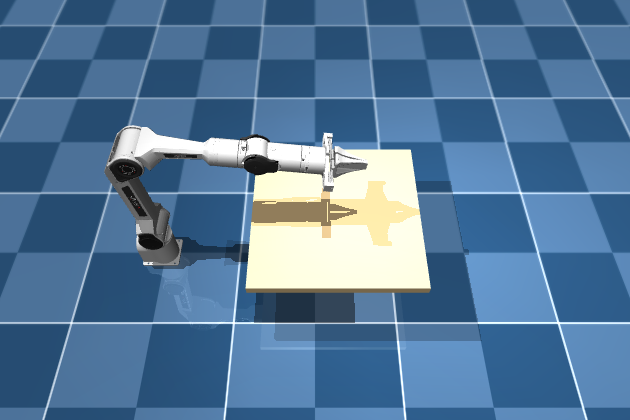
\includegraphics[width=0.85\columnwidth]{figures/pickbench_render.png}
\caption{The pickbench scene used for the Piper end-to-end Pick
experiment (\S\ref{sec:cap-cross-robot}). Three graspable cubes
(red, green, blue) sit on a 20\,cm $\times$ 20\,cm table within
Piper's reachable workspace.}
\label{fig:pickbench}
\end{figure}

\section{Bedrock model identifiers and pricing}
\label{app:models}

All LLM-agent experiments run against AWS Bedrock. Anthropic
models use the native tool-use API; the other four vendors use the
unified Bedrock Converse API through a thin adapter, so the agent
loop is identical across vendors. Table~\ref{tab:bedrock} lists
exact identifiers and per-token pricing used for all cost figures.

\begin{table*}[t]
\centering
\small
\begin{tabular}{llll}
\toprule
\textbf{Label} & \textbf{Vendor} & \textbf{Bedrock identifier} & \textbf{Pricing (per 1M tok, in/out)} \\
\midrule
Haiku~4.5     & Anthropic & \texttt{us.anthropic.claude-haiku-4-5-20251001-v1:0}  & \$1.00 / \$5.00 \\
Sonnet~4.5    & Anthropic & \texttt{us.anthropic.claude-sonnet-4-5-20250929-v1:0} & \$3.00 / \$15.00 \\
Sonnet~4.6    & Anthropic & \texttt{us.anthropic.claude-sonnet-4-6}               & \$3.00 / \$15.00 \\
Opus~4.8      & Anthropic & \texttt{us.anthropic.claude-opus-4-8}                 & \$5.00 / \$25.00 \\
Nova~Pro      & Amazon    & \texttt{amazon.nova-pro-v1:0}                         & \$0.80 / \$3.20 \\
DeepSeek~V3.2 & DeepSeek  & \texttt{deepseek.v3.2}                                & \$0.27 / \$1.10 \\
Ministral~8B  & Mistral   & \texttt{mistral.ministral-3-8b-instruct}             & \$0.10 / \$0.10 \\
Qwen3~32B     & Alibaba   & \texttt{qwen.qwen3-32b-v1:0}                          & \$0.15 / \$0.60 \\
\bottomrule
\end{tabular}
\caption{The eight Bedrock models (five vendors) and their
per-token list pricing as of May 2026, used for all cost figures in
the paper.}
\label{tab:bedrock}
\end{table*}

Across the leaderboard runs of
\S\ref{sec:cap-portability} (seven models, using and synthesizing
conditions), the agents consumed 25.4M input and 882k output tokens in total;
per-configuration token counts are stored in each result JSON.
The synthesis pipeline (\S\ref{sec:onboarding}) uses Sonnet~4.5 as
its default agent. The cross-model capability study
(\S\ref{sec:cap-portability}) sweeps all seven of the other models
above on the full 13-task SO-101 suite; smaller open-weight models
(Ministral~8B, Qwen3~32B) and a strong open model (DeepSeek~V3.2)
are included to test whether synthesis is restricted to the
strongest closed models.
Gemma-3 and Llama-3/4 were excluded after a tool-use smoke test:
Gemma-3-27B does not emit Converse tool calls, and the Llama
endpoints required an inference profile not available in our
account.

Figure~\ref{fig:cost-quality} combines this pricing with the
\S\ref{sec:cap-portability} leaderboard into a single cost--quality
plane: each point is one model $\times$ method configuration over
the full 13-task suite at $N{=}5$.

\begin{figure}[t]
\centering
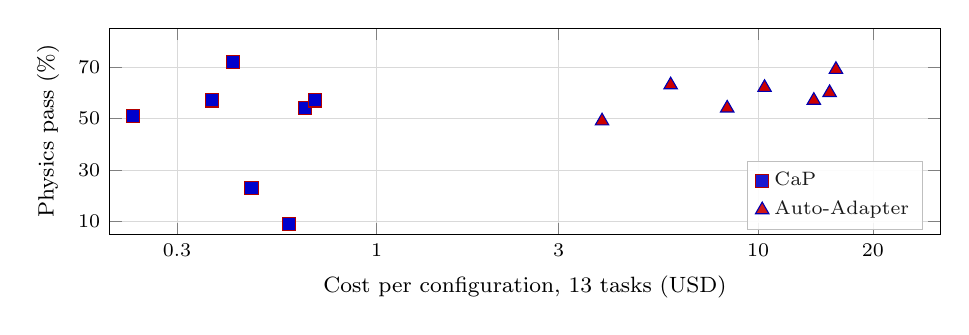
\begin{tikzpicture}
\begin{axis}[
  width=\columnwidth,
  height=4.2cm,
  xmode=log,
  log basis x=10,
  xlabel={\footnotesize Cost per configuration, 13 tasks (USD)},
  ylabel={\footnotesize Physics pass (\%)},
  xmin=0.2, xmax=30,
  ymin=5, ymax=85,
  xtick={0.3,1,3,10,20},
  xticklabels={0.3,1,3,10,20},
  ytick={10,30,50,70},
  grid=both,
  major grid style={line width=0.1pt, draw=gray!30},
  minor grid style={line width=0.05pt, draw=gray!15},
  tick label style={font=\scriptsize},
  legend style={font=\scriptsize, at={(0.98,0.02)}, anchor=south east,
                draw=gray!50, fill=white, fill opacity=0.9},
  legend cell align={left},
]
% CaP series (cost, phys): 7 models
\addplot+[only marks, mark=square*, mark size=2.4pt,
          draw=red!70!black, fill=red!40]
  coordinates {(0.65,54) (0.69,57) (0.23,51) (0.37,57) (0.59,9) (0.47,23) (0.42,72)};
\addlegendentry{CaP}
% Auto-Adapter series (cost, phys): 7 models
\addplot+[only marks, mark=triangle*, mark size=2.8pt,
          draw=blue!70!black, fill=blue!40]
  coordinates {(10.4,62) (16.0,69) (5.9,63) (15.4,60) (14.0,57) (8.3,54) (3.9,49)};
\addlegendentry{Auto-Adapter}
\end{axis}
\end{tikzpicture}
\caption{Cost--quality on the full 13-task SO-101 suite, seven
models $\times$ two methods (\S\ref{sec:cap-portability}).
Triangles (ours) occupy a higher-success, higher-cost regime;
squares (CaP) are cheap but high-variance (the high CaP outlier is
Qwen3~32B). Cost is per 13-task configuration at $N{=}5$.}
\label{fig:cost-quality}
\end{figure}


\section{Task execution filmstrips}
\label{app:filmstrips}

Each row below is a single trial of the agent-synthesized driver
executing a real task in MuJoCo, captured at five time points. The
SO-101 Reach and Piper Pick strips are deterministic rollouts of
the synthesized driver's own \texttt{move\_cartesian} and
\texttt{gripper\_close} primitives. The SO-101 \texttt{draw\_letter\_L}
strip re-executes the graded down-4\,cm/forward-4\,cm L trajectory
of the hard-suite task (\S\ref{sec:cap-portability}) through the
synthesized driver's own IK. The Go2, Skydio~X2, H1, and
ANYmal-C strips execute the respective drivers' primitives live in
MuJoCo (\texttt{sit}/\texttt{stand\_up};
\texttt{takeoff}/\texttt{move\_to}/\texttt{land}; \texttt{squat};
\texttt{walk\_forward}), covering all four morphology classes the
pipeline targets (Appendix~\ref{app:morphology}).

\begin{figure*}[t]
\centering
\setlength{\tabcolsep}{1pt}
\renewcommand{\arraystretch}{0.3}
\begin{tabular}{ccccc}
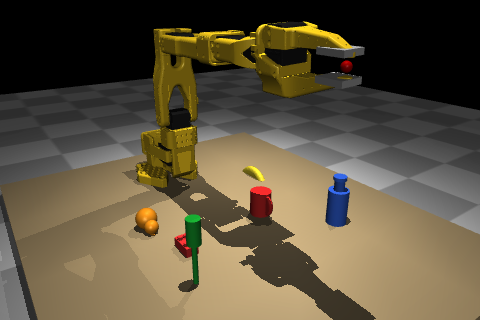
\includegraphics[width=0.18\textwidth]{figures/film_so101_reach_0.png} &
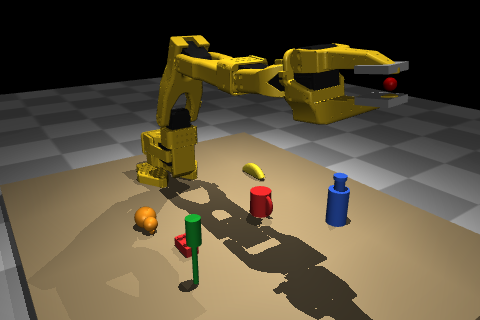
\includegraphics[width=0.18\textwidth]{figures/film_so101_reach_1.png} &
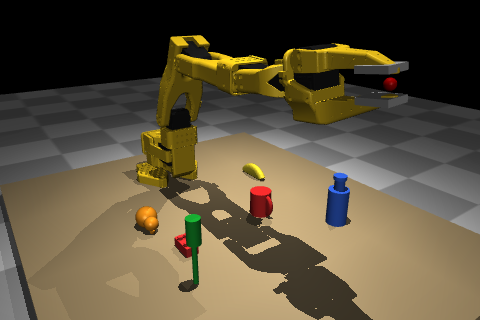
\includegraphics[width=0.18\textwidth]{figures/film_so101_reach_2.png} &
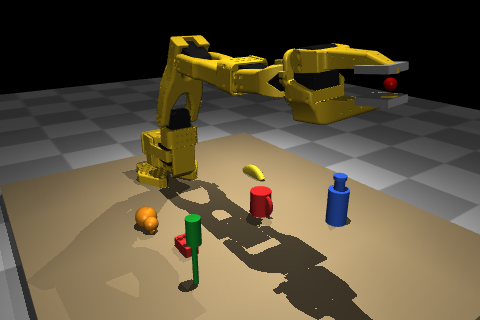
\includegraphics[width=0.18\textwidth]{figures/film_so101_reach_3.png} &
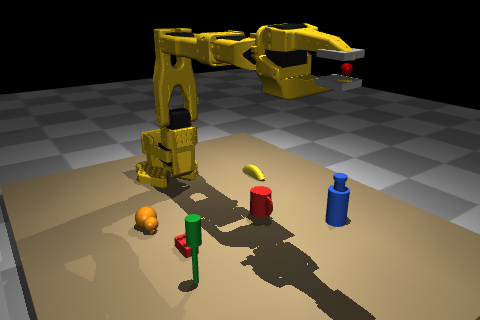
\includegraphics[width=0.18\textwidth]{figures/film_so101_reach_4.png} \\
\multicolumn{5}{c}{\parbox{0.92\textwidth}{\small\textbf{(a) SO-101 \texttt{reach\_x+5}.}
Home $\rightarrow$ 33\% $\rightarrow$ 66\% $\rightarrow$ at target $\rightarrow$ return-to-home.
$N{=}10$ trials, 10/10 pass (\S\ref{sec:cap-cross}, Table~\ref{tab:cross-skill}).}} \\[6pt]

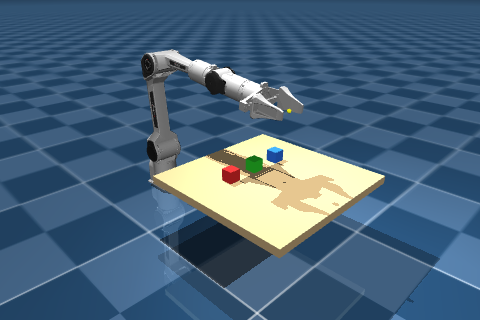
\includegraphics[width=0.18\textwidth]{figures/film_piper_pick_0.png} &
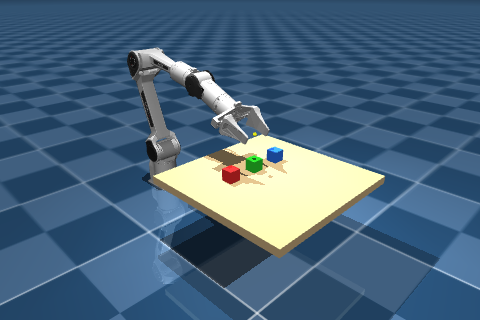
\includegraphics[width=0.18\textwidth]{figures/film_piper_pick_1.png} &
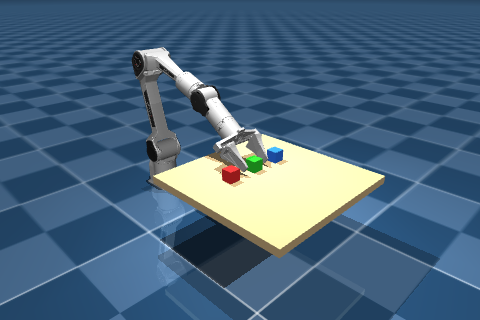
\includegraphics[width=0.18\textwidth]{figures/film_piper_pick_2.png} &
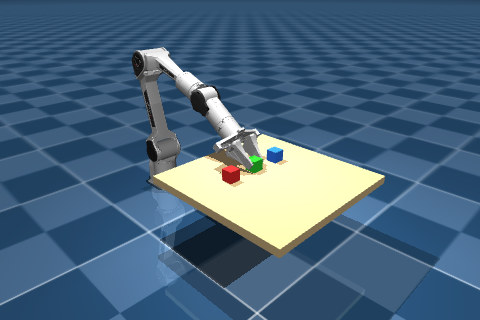
\includegraphics[width=0.18\textwidth]{figures/film_piper_pick_3.png} &
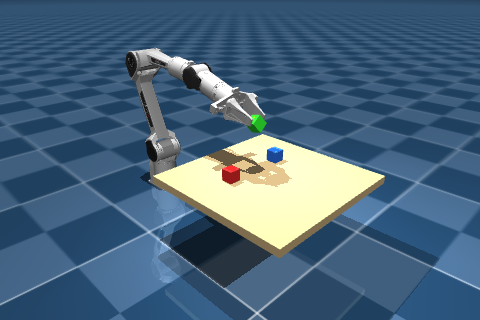
\includegraphics[width=0.18\textwidth]{figures/film_piper_pick_4.png} \\
\multicolumn{5}{c}{\parbox{0.92\textwidth}{\small\textbf{(b) Piper \texttt{pick\_green}.}
Home (gripper open) $\rightarrow$ 8\,cm pre-grasp $\rightarrow$
lower to the cube $\rightarrow$ \texttt{gripper\_close} (weld to cube)
$\rightarrow$ lift 12\,cm. The agent-written \texttt{gripper\_close}
does the distance check and weld activation; the 13-line
post-synthesis patch adds \texttt{get\_object\_position} and the
weld relpose update (\S\ref{sec:cap-cross-robot}).}} \\[6pt]

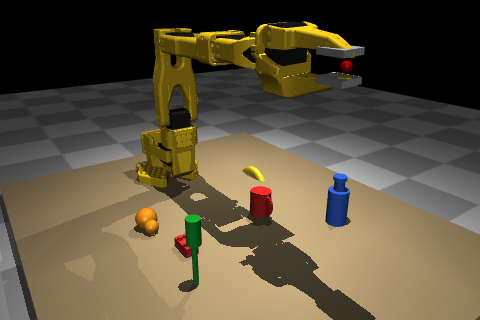
\includegraphics[width=0.18\textwidth]{figures/film_so101_letter_0.png} &
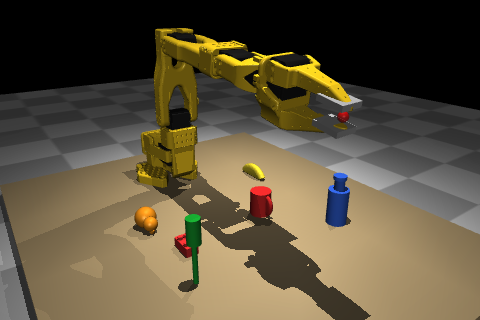
\includegraphics[width=0.18\textwidth]{figures/film_so101_letter_1.png} &
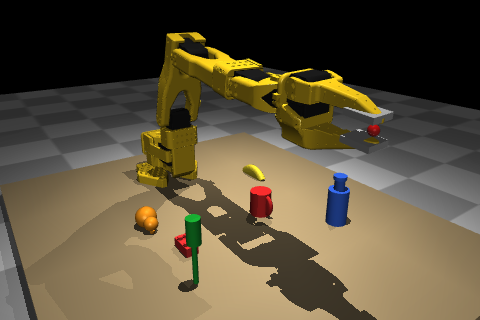
\includegraphics[width=0.18\textwidth]{figures/film_so101_letter_2.png} &
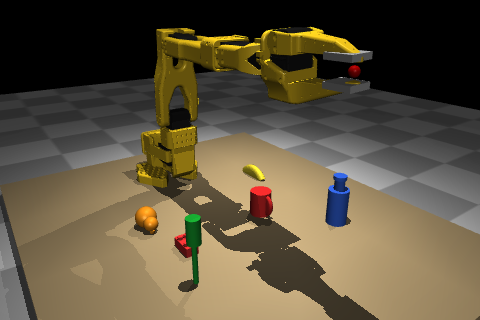
\includegraphics[width=0.18\textwidth]{figures/film_so101_letter_3.png} &
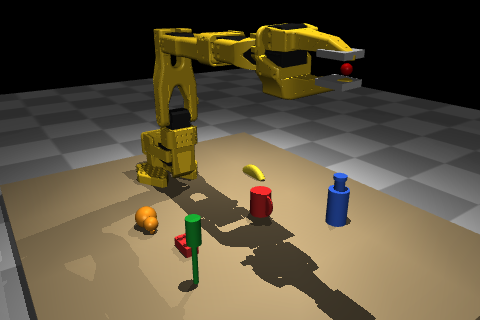
\includegraphics[width=0.18\textwidth]{figures/film_so101_letter_4.png} \\
\multicolumn{5}{c}{\parbox{0.92\textwidth}{\small\textbf{(c) SO-101 \texttt{draw\_letter\_L}}
(hard suite; graded trajectory re-executed by the synthesized driver). A two-leg L within the
SO-101 workspace: 4\,cm down, then 4\,cm forward ($+X$), then return
home. Graded by \texttt{ee\_waypoint\_trace}, which verifies the
end-effector actually visits both corners (in order) and returns
home, not merely the return. $N{=}5$ per model,
\S\ref{sec:cap-portability}.}} \\[6pt]

\multicolumn{1}{c}{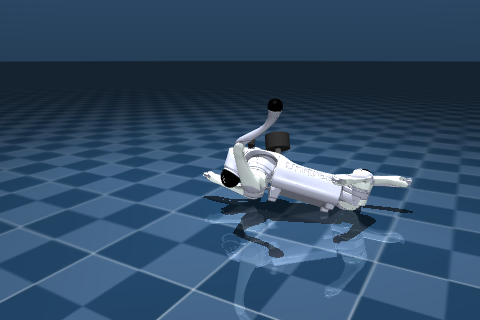
\includegraphics[width=0.18\textwidth]{figures/film_go2_walk_0.png}} &
\multicolumn{1}{c}{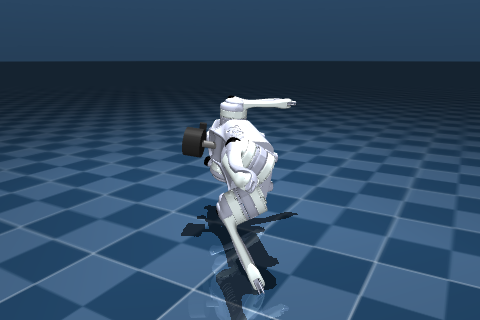
\includegraphics[width=0.18\textwidth]{figures/film_go2_walk_1.png}} &
\multicolumn{1}{c}{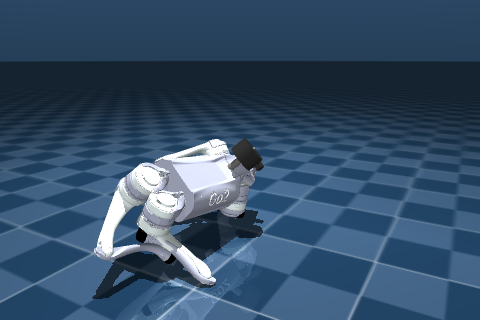
\includegraphics[width=0.18\textwidth]{figures/film_go2_walk_2.png}} &
\multicolumn{1}{c}{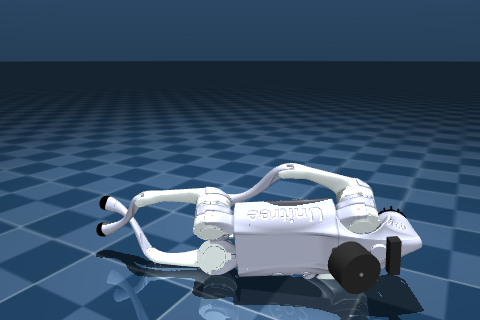
\includegraphics[width=0.18\textwidth]{figures/film_go2_walk_3.png}} &
\multicolumn{1}{c}{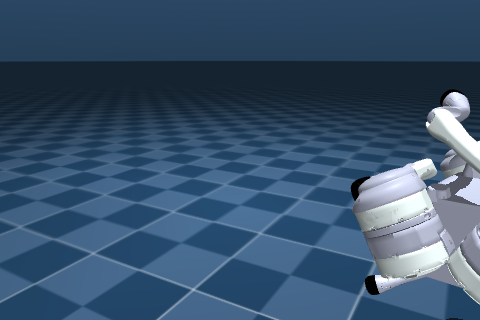
\includegraphics[width=0.18\textwidth]{figures/film_go2_walk_4.png}} \\
\multicolumn{5}{c}{\parbox{0.92\textwidth}{\small\textbf{(d) Go2 \texttt{sit} $\rightarrow$ \texttt{stand\_up} attempt}
(driver primitives executed live). The visible instability is the
point: the driver passes the 8/8 onboarding validation
(Table~\ref{tab:onboarding-detail}), yet the independent smoke
suite scores \texttt{stand\_up} 0/2 (Appendix~\ref{app:smoke}): the
validator-leniency gap disclosed in Appendix~\ref{app:onboarding},
and the reason every \S\ref{sec:capability} number is graded by
independent physics, never by the onboarding harness.}} \\
\end{tabular}
\caption{Task-execution filmstrips (manipulation and Go2). Five
frames per row, captured at evenly-spaced time points during a
single rollout of the agent-synthesized driver. Underlying
simulator is MuJoCo (\S\ref{sec:protocol}). All frames are
produced from the same artifacts that drive the quantitative
results in the body of the paper.}
\label{fig:filmstrips}
\end{figure*}

\begin{figure*}[t]
\centering
\setlength{\tabcolsep}{1pt}
\renewcommand{\arraystretch}{0.3}
\begin{tabular}{ccccc}
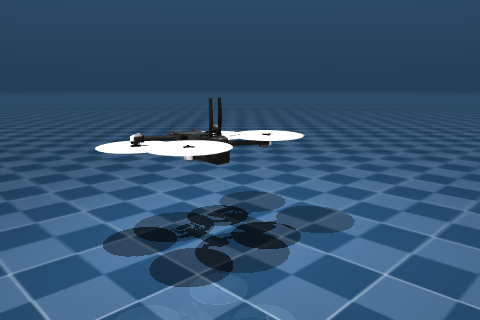
\includegraphics[width=0.18\textwidth]{figures/film_skydio_0.png} &
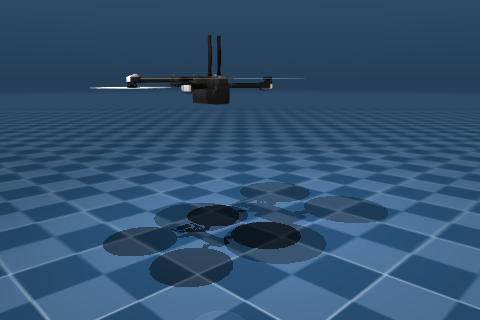
\includegraphics[width=0.18\textwidth]{figures/film_skydio_1.png} &
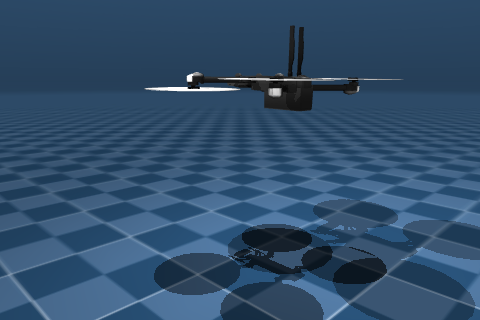
\includegraphics[width=0.18\textwidth]{figures/film_skydio_2.png} &
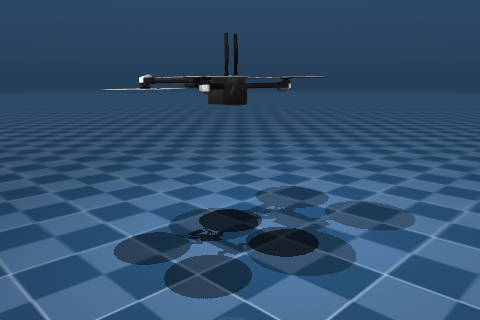
\includegraphics[width=0.18\textwidth]{figures/film_skydio_3.png} &
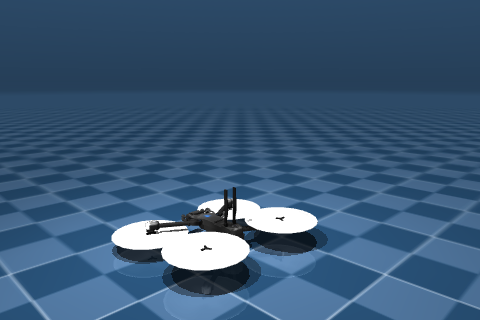
\includegraphics[width=0.18\textwidth]{figures/film_skydio_4.png} \\
\multicolumn{5}{c}{\parbox{0.92\textwidth}{\small\textbf{(e) Skydio~X2 quadrotor go-to}
(aerial suite, Appendix~\ref{app:morphology}). Ground $\rightarrow$
\texttt{takeoff} to 0.5\,m $\rightarrow$ \texttt{move\_to}
$(0.4, 0, 0.5)$ $\rightarrow$ return $\rightarrow$ \texttt{land}.
The cascaded position$\rightarrow$attitude$\rightarrow$thrust
controller is synthesized zero-shot from the MJCF; both agent
styles score $8/8$ on the hardened aerial suite
(Table~\ref{tab:aerial}).}} \\[6pt]

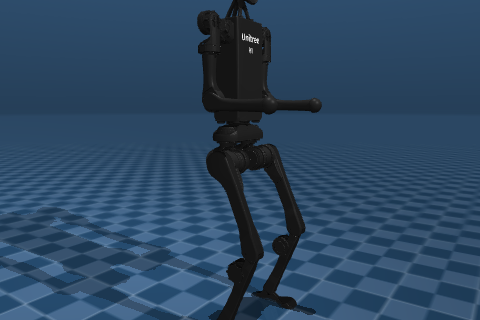
\includegraphics[width=0.18\textwidth]{figures/film_h1_0.png} &
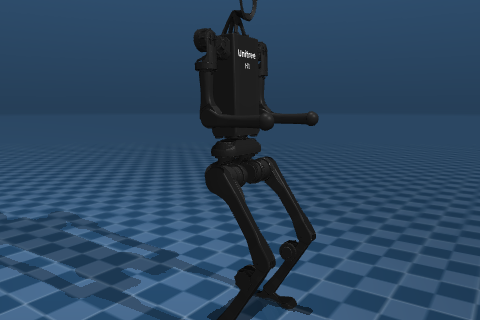
\includegraphics[width=0.18\textwidth]{figures/film_h1_1.png} &
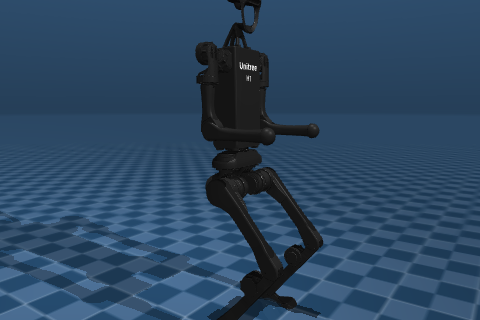
\includegraphics[width=0.18\textwidth]{figures/film_h1_2.png} &
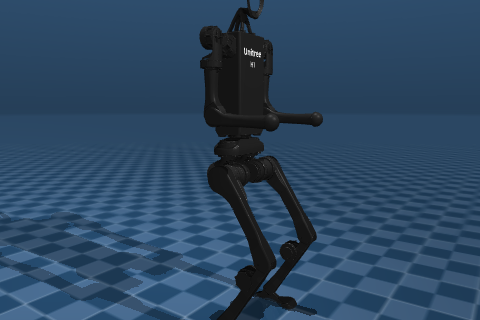
\includegraphics[width=0.18\textwidth]{figures/film_h1_3.png} &
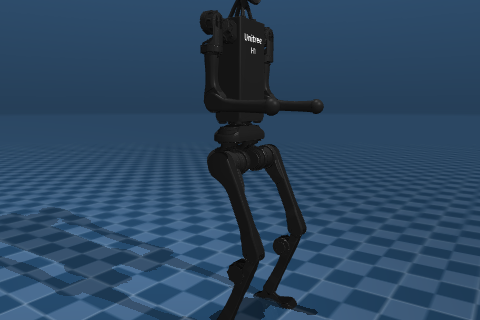
\includegraphics[width=0.18\textwidth]{figures/film_h1_4.png} \\
\multicolumn{5}{c}{\parbox{0.92\textwidth}{\small\textbf{(f) H1 humanoid squat-recover}
(Appendix~\ref{app:morphology}). The 19-DoF biped holds a PD-balanced
stand, bends at the knees and hips, and recovers without falling over;
the motion is deliberately conservative (torso dips from
0.98\,m and returns to 0.97\,m), which is what the validated
\texttt{squat} primitive does; dynamic walking remains the
pipeline's hardest open case (Appendix~\ref{app:morphology}).}} \\[6pt]

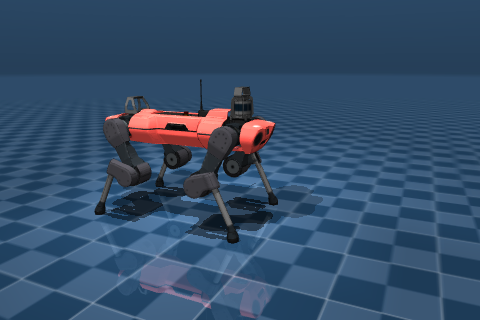
\includegraphics[width=0.18\textwidth]{figures/film_anymal_0.png} &
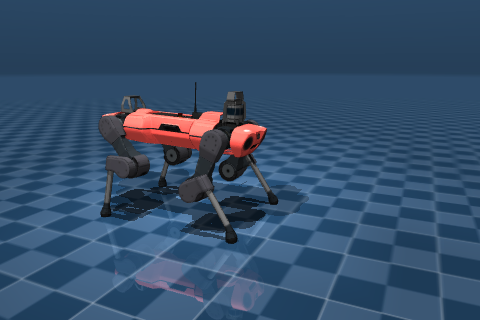
\includegraphics[width=0.18\textwidth]{figures/film_anymal_1.png} &
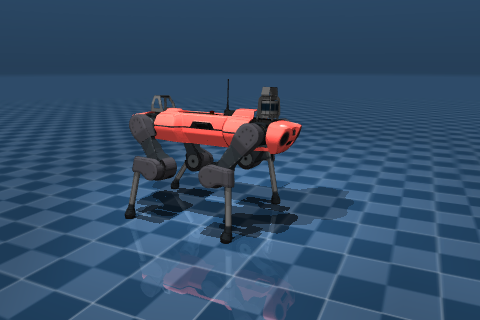
\includegraphics[width=0.18\textwidth]{figures/film_anymal_2.png} &
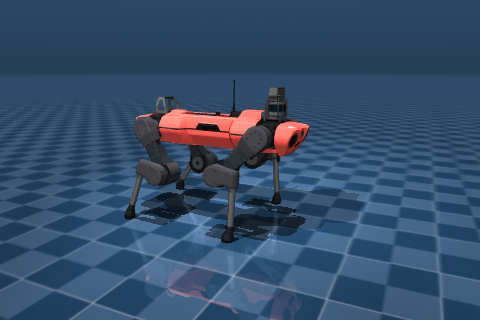
\includegraphics[width=0.18\textwidth]{figures/film_anymal_3.png} &
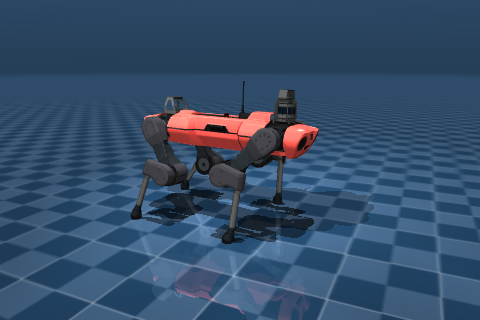
\includegraphics[width=0.18\textwidth]{figures/film_anymal_4.png} \\
\multicolumn{5}{c}{\parbox{0.92\textwidth}{\small\textbf{(g) ANYmal-C \texttt{walk\_forward}}
(locomotion v2 suite, \S\ref{sec:cap-cross-robot}). Stand, then four
2\,s \texttt{walk\_forward} calls at speed 0.2, the same call
pattern as the graded eval trials; the base advances 0.24\,m while
holding ${\approx}0.5$\,m body height. Executed live on the shared
driver behind the \S\ref{sec:cap-cross-robot} locomotion
comparison, where ANYmal-C favors Auto-Adapter (68\% vs.\ 28\%).}} \\
\end{tabular}
\caption{Morphology-breadth filmstrips (aerial, humanoid,
quadruped walking), rendered as in Figure~\ref{fig:filmstrips}.}
\label{fig:filmstrips2}
\end{figure*}

\section{Per-phase pipeline gallery}
\label{app:gallery}

This appendix walks through one concrete pass of the
\S\ref{sec:pipeline} pipeline on SO-101, showing the actual
artifact produced at each phase. All artifacts shown are reproduced
verbatim from the SO-101 run logged in
\texttt{artifacts/auto\_adapter\_from\_}\allowbreak\texttt{scratch\_so101\_artifacts/}
(referenced throughout the body of the paper).

\subsection{Phase 1: STUDY (parse MJCF, emit Spec)}

The agent reads \texttt{mjcf.xml}, identifies actuators and joints,
and writes a structured Spec object summarizing the robot's degrees
of freedom and limits. Excerpt:

\begin{lstlisting}[basicstyle=\ttfamily\scriptsize, frame=single, framerule=0pt,
    backgroundcolor=\color{gray!10}, columns=fullflexible, breaklines=true]
{
  "robot_id": "so101_from_scratch",
  "estimated_class": "arm",
  "dof": 5,
  "arm_joint_names": ["shoulder_pan", "shoulder_lift",
                      "elbow_flex", "wrist_flex", "wrist_roll"],
  "joint_limits": {
    "shoulder_pan":   [-1.92, 1.92],
    "shoulder_lift":  [-1.75, 1.75],
    "elbow_flex":     [-1.69, 1.69],
    "wrist_flex":     [-1.66, 1.66],
    "wrist_roll":     [-2.74, 2.84]
  },
  "ee_site": "ee_site",
  "ee_body": "gripper_link",
  "gripper_actuator_names": ["act_jaw_visual"],
  "actuator_type_hint": "position"
}
\end{lstlisting}

\subsection{Phase 2: GENERATE (Spec $\rightarrow$ driver code)}

The agent emits \texttt{driver\_from\_scratch.py}: 546 lines of
self-contained Python that exposes \texttt{home}, \texttt{move\_cartesian},
\texttt{gripper\_open}, \texttt{gripper\_close}, etc. The
inverse-kinematics inner loop, written by the agent without any
skeleton library, is reproduced below:

\begin{lstlisting}[basicstyle=\ttfamily\scriptsize, frame=single, framerule=0pt,
    backgroundcolor=\color{gray!10}, columns=fullflexible, breaklines=true,
    language=Python]
for iteration in range(max_iter):
    self.set_joint_positions(q)
    mujoco.mj_forward(self.model, self.data)
    current_xyz = self.data.site_xpos[self.site_id].copy()
    error = target_xyz - current_xyz
    if np.linalg.norm(error) < tol:
        return q, True, np.linalg.norm(error)

    J = self.compute_jacobian()
    # Adaptive damping: scales with error magnitude
    lambda_damping = self.ik_lambda_base * (1.0 + np.linalg.norm(error))
    JtJ = J.T @ J + lambda_damping**2 * np.eye(self.n_joints)
    dq = np.linalg.solve(JtJ, J.T @ error)
    # Step-size control prevents overshoot in poorly-conditioned regions
    step = min(1.0, 0.5 / (np.linalg.norm(dq) + 1e-6))
    q += step * dq
    q = self._clamp_to_limits(q)
\end{lstlisting}

Damped Least Squares with adaptive $\lambda$ and step-size clamping
is a textbook IK formulation, here written from scratch by the
agent against the per-robot Spec produced in Phase~1. The choice
is deliberate rather than a limitation: DLS stays well-behaved
near singularities and needs nothing beyond \texttt{numpy},
matching the self-contained delivery constraint (\S\ref{sec:modes}).

\subsection{Phase 3: VALIDATE (run the harness)}

The driver is imported and exercised against a fixed,
robot-class-aware test suite. SO-101's seven tests are reproduced
verbatim from \texttt{validate\_report.json} in Table~\ref{tab:validate}:

\begin{table}[H]
\centering
\small
\begin{tabular}{llr}
\toprule
\textbf{Test} & \textbf{Status} & \textbf{Metric} \\
\midrule
no\_skeleton\_import  & OK & --- \\
robot\_class\_present & OK & --- \\
build\_from\_mjcf     & OK & --- \\
home                  & OK & --- \\
ik\_roundtrip         & OK & 9.67\,mm err \\
gripper\_cycle        & OK & --- \\
describe              & OK & --- \\
\bottomrule
\end{tabular}
\caption{SO-101 validate-phase output (7/7); exact contents of
\texttt{artifacts/.../validate\_report.json}.}
\label{tab:validate}
\end{table}

If any test fails, the orchestrator re-enters Phase~2 with the
failure surfaced as a structured error in the prompt
(Appendix~\ref{app:reliability} reports the controlled rerun showing the
loop converges at outer iteration~1 on SO-101).

\subsection{Phase 4: EXPORT (package the artifact)}

A directory snapshot is captured for downstream consumption. The
SO-101 artifact tree:

\begin{lstlisting}[basicstyle=\ttfamily\scriptsize, frame=single, framerule=0pt,
    backgroundcolor=\color{gray!10}, columns=fullflexible]
artifacts/auto_adapter_from_scratch_so101_artifacts/
|-- driver_from_scratch.py    # 546 lines, agent-written
|-- mjcf.xml                  # symlink to assets/mjcf/so101_*.xml
|-- study.json                # Phase 1 output (Spec)
|-- validate_report.json      # Phase 3 output (test results)
\-- IMPLEMENTATION_SUMMARY.md # agent-written narrative
\end{lstlisting}

\subsection{Phase 5: DEMO (rendered execution)}

The exported driver is exercised by a small demo script (\texttt{home()}
then a reach target then \texttt{home()}) and the rollout is rendered
frame by frame. Figure~\ref{fig:demo-frame} shows the rollout at
the moment the end-effector reaches its target. The
full filmstrip for this same task is row (a) of
Figure~\ref{fig:filmstrips} in Appendix~\ref{app:filmstrips};
Appendix~\ref{app:traces} gives a side-by-side Auto-Adapter vs.\
Code-as-Policies trace for one task.

\begin{figure}[H]
\centering
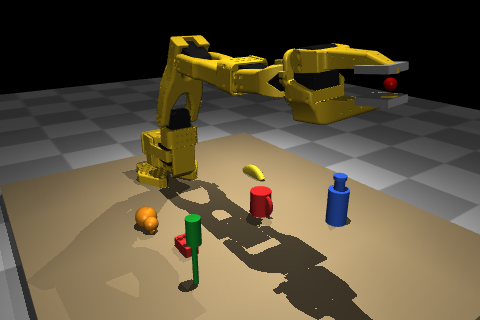
\includegraphics[width=0.7\columnwidth]{figures/film_so101_reach_3.png}
\caption{SO-101 demo frame at \texttt{reach\_x+5} target position
(end-effector at home$+5$\,cm in X, in MuJoCo). The synthesized
driver's \texttt{move\_cartesian} produced the trajectory. Compare
against Figure~\ref{fig:filmstrips}(a) for the full rollout.}
\label{fig:demo-frame}
\end{figure}

\section{Grader taxonomy}
\label{app:graders}

\begin{table}[H]
\centering
\footnotesize
\setlength{\tabcolsep}{1.5pt}
\begin{tabular}{@{}lcll@{}}
\toprule
\textbf{Suite} & \textbf{Loc.} & \textbf{Robot} & \textbf{Tasks} \\
\midrule
Cross-skill       & 5.1 & SO-101       & 4 reach, 10 pick \\
Multi-task         & 5.2 & SO-101       & 6 dirs + 4 held-out \\
Hard suite        & 5.3 & SO-101       & 12 phys + 1 cov \\
Simple suite      & 5.4 & Piper, UR5e  & 5 short tasks \\
Piper Pick        & 5.4 & Piper        & 3 reach + 3 pick \\
OpenVLA reach     & \ref{app:openvla-sweep} & SO-101 & 5 reach (RGB) \\
Locomotion v2     & 5.4 & Go2, ANYmal-C & 10 loco tasks \\
\bottomrule
\end{tabular}
\caption{Downstream task suites (\S\ref{sec:capability}). Reach suites
run 10 trials per offset; the hard suite is 12 physics-graded plus 1
coverage task.}
\label{tab:suites}
\end{table}

\noindent\textbf{Grader taxonomy.} AutoAdapter-Bench implements 42
grader types in \texttt{eval.py}; 31 are exercised by the released
task suites. Twenty-eight of those 31 read \emph{post-step simulator
state}: end-effector pose (\texttt{ee\_at\_midpoint},
\texttt{ee\_waypoint\_trace}), object pose and contact
(\texttt{object\_above\_object}, \texttt{object\_lifted\_by},
\texttt{objects\_swapped}, \texttt{object\_pose\_match\_relative}),
body height (\texttt{body\_height\_ratio}), and base pose/yaw for
locomotion (\texttt{forward\_progress}, \texttt{turn\_to\_heading},
\texttt{drive\_and\_turn}). The remaining three are deliberately
\emph{behavioral}, and we label them as such rather than fold them
into the physics count: failure-detection
(\texttt{llm\_reports\_failure}, used by \texttt{unreachable\_detect},
where the correct behavior is to \emph{report} an
\texttt{IKUnreachableError} rather than move), tool-liveness
(\texttt{tool\_executed\_without\_crash}, used by
\texttt{gripper\_cycle}), and end-effector coverage
(\texttt{ee\_visited\_n\_positions}, used by
\texttt{visit\_all\_objects}). The first two sit in the simple suite
(\S\ref{sec:cap-cross-robot}); only the third,
\texttt{visit\_all\_objects}, sits in the 13-task hard suite. In the
released code \texttt{ee\_visited\_n\_positions} now verifies that the
end-effector physically came within tolerance of each object's true
world position (falling back to commanded-target coverage only when
the per-call trajectory is unavailable).

\noindent\textbf{Grasp grading.} For grasp tasks,
\texttt{object\_lifted\_by} requires the target to be both lifted
\emph{and} still held within 12\,cm of the end-effector at the final
step, rejecting an object flung by a faulty weld constraint that would
pass a height-only check. The self-contained validation suite includes
a matching \texttt{grasp\_lift} test, so a driver that cannot truly
grasp fails synthesis rather than inflating its Self score.

\section{12-task robustness and statistical tests}
\label{app:robustness}

\noindent\textbf{12-task physics-only robustness.} The single
behavioral task in the hard suite is \texttt{visit\_all\_objects}.
Table~\ref{tab:robustness} reports the SO-101 portability comparison
on the 12 physics-graded tasks alone (dropping that one task), using
the same trials. The model ranking is unchanged: Auto-Adapter beats
zero-shot CaP on six of seven models and beats few-shot CaP on four
(tying Haiku), exactly as on the full 13-task suite
(Table~\ref{tab:portability}). The headline therefore does not depend
on the behavioral task or on how it is graded.

\begin{table}[H]
\centering
\small
\begin{tabular}{lrrrr}
\toprule
\textbf{Model} & \textbf{A-A} & \textbf{CaP} & \textbf{CaP\textsubscript{fs}} & \textbf{Self} \\
\midrule
Sonnet~4.6    & \textbf{67} & 53 & 50 & -- \\
Opus~4.8      & \textbf{60} & 47 & 45 & 42 \\
Haiku~4.5     & \textbf{58} & 50 & \textbf{58} & 42 \\
Nova~Pro      & \textbf{57} & 53 & 42 & -- \\
DeepSeek~V3.2 & 53          & 10 & \textbf{57} & 22 \\
Ministral~8B  & \textbf{50} & 25 & 38 & -- \\
Qwen3~32B     & 45          & \textbf{70} & 53 & -- \\
\bottomrule
\end{tabular}
\caption{SO-101 portability on the \textbf{12 physics-graded} hard-suite
tasks (\texttt{visit\_all\_objects} excluded), \%, $N{=}5$ trial-level.
Bold = best of A-A/CaP/CaP\textsubscript{fs}. Ranking matches the
13-task Table~\ref{tab:portability}: A-A $>$ CaP on 6/7; A-A $>$
CaP\textsubscript{fs} on 4/7 (Haiku tie).}
\label{tab:robustness}
\end{table}

\noindent\textbf{Statistical significance.} \textbf{In brief: the
Auto-Adapter advantage over zero-shot CaP is significant at the
task level, but individual per-model cells are not separately
resolvable at $N{=}5$.} We test Auto-Adapter vs.\
zero-shot CaP with the (model, task) cell as the paired unit (seven
models $\times$ 13 tasks, $n{=}91$ cells; $N{=}5$ trials each), computed
by \texttt{autoadapter\_bench/stats.py}. Auto-Adapter leads by a mean
$+13.0$ points per cell, and a Wilcoxon signed-rank test over the paired
cells is significant ($W{=}138$, $p{<}0.01$; pooled trial rate $0.59$
vs.\ $0.46$). The coarser model-level comparison over the seven
aggregate rates is only suggestive ($+13$ pp mean; sign test $p{=}0.13$,
Wilcoxon $p{=}0.15$; $n{=}7$ is underpowered), so we rest the claim on
the task-level test rather than on the 6/7 win count. Against few-shot
CaP the aggregate effect is \emph{not} significant ($p{=}0.13$), so we
report that comparison descriptively only. Per cell, only the two
largest gaps clear non-overlapping 95\% Wilson intervals (DeepSeek A-A
$0.57\,[0.45,0.68]$ vs.\ CaP $0.09\,[0.04,0.19]$; Ministral A-A
$0.54\,[0.42,0.65]$ vs.\ CaP $0.23\,[0.15,0.35]$); for the four closely matched Anthropic/Nova cells the per-model
intervals overlap. The effect is therefore robust in aggregate but, at
$N{=}5$, individual cell differences below ${\sim}15$ points are not
separately resolvable, so we do not claim per-model significance.

\noindent\textbf{Quadruped agent-model ablation.} The
\S\ref{sec:cap-cross-robot} quadruped numbers use a Sonnet~4.5 agent
on a shared Sonnet~4.5 driver. Re-running the same 10-task suite with
a Sonnet~4.6 agent gives the same qualitative split (ANYmal-C
favors Auto-Adapter, Go2 reverses), consistent with an
embodiment-driven rather than agent-version-driven effect
(Table~\ref{tab:quad-ablation}).

\begin{table}[H]
\centering
\small
\begin{tabular}{llrr}
\toprule
\textbf{Robot} & \textbf{Agent} & \textbf{A-A} & \textbf{CaP} \\
\midrule
ANYmal-C & Sonnet~4.5 & \textbf{68} & 28 \\
ANYmal-C & Sonnet~4.6 & \textbf{62} & 50 \\
Go2      & Sonnet~4.5 & 48 & \textbf{54} \\
Go2      & Sonnet~4.6 & 44 & \textbf{54} \\
\bottomrule
\end{tabular}
\caption{Quadruped locomotion (10-task v2 suite, physics \%, $N{=}5$):
Sonnet~4.5 (main, \S\ref{sec:cap-cross-robot}) vs.\ Sonnet~4.6
(ablation). The ANYmal-favors-A-A / Go2-reverses split holds under
both agent versions.}
\label{tab:quad-ablation}
\end{table}

\subsection{Pretrained-VLA probe: OpenVLA-7B zero-shot on SO-101}
\label{app:openvla-sweep}

As an auxiliary check we ran a pretrained vision-language-action model,
OpenVLA-7B, zero-shot on the five SO-101 reach variants
(50 episodes). This is a cross-embodiment \emph{probe}, not a
like-for-like baseline: OpenVLA reads RGB rather than the privileged
state our agent and the RL/CaP baselines use, SO-101 is not in its
Open-X training mixture, and its camera frame differs from training; we
therefore keep it out of the main comparison. It scores \textbf{0/50}
(mean EE error 23\,cm, deltas in inconsistent directions), consistent
with the per-embodiment finetuning OpenVLA requires
\citep[\S 3]{kim2024openvla}. Because a zero invites the objection that
the action adapter, not the model, failed, we validate the harness and
sweep the two configuration knobs a reviewer would question. \emph{Harness validation:} an oracle that feeds
the ground-truth direction (target $-$ current EE) through the identical
\texttt{move\_cartesian} path reaches all five reach targets (5/5, mean
final error 1.3\,cm) at the per-step control budget used for OpenVLA
(\texttt{duration}{=}0.5\,s); the same path with a shorter
\texttt{duration} (0.1\,s) reaches 0/5. A capable
controller therefore passes on this harness, so a model score of 0 is a
model result. \emph{Robustness:} Table~\ref{tab:openvla-sweep} sweeps
six action scales (0.25--10$\times$) and eight \texttt{unnorm}
de-normalization keys OpenVLA-7B ships (\texttt{bridge\_orig} plus
seven others, the manipulation datasets closest to SO-101). Every cell is $\leq$6.7\% (one chance episode of
15), so the failure is not an artifact of one de-normalization or scale
choice.

\begin{table}[H]
\centering
\small
\setlength{\tabcolsep}{4pt}
\begin{tabular}{llrr}
\toprule
\textbf{unnorm key} & \textbf{scale} & \textbf{success} & \textbf{err (cm)} \\
\midrule
bridge\_orig & 0.25 & 0.0\% & 10.3 \\
bridge\_orig & 0.50 & 0.0\% & 13.1 \\
bridge\_orig & 1.00 & 6.7\% & 15.3 \\
bridge\_orig & 2.00 & 0.0\% & 23.8 \\
bridge\_orig & 5.00 & 0.0\% & 33.7 \\
bridge\_orig & 10.0 & 0.0\% & 47.0 \\
\midrule
fractal20220817\_data & 2.00 & 0.0\% & 58.4 \\
berkeley\_autolab\_ur5 & 2.00 & 0.0\% & 18.7 \\
taco\_play & 2.00 & 0.0\% & 50.2 \\
jaco\_play & 2.00 & 0.0\% & 54.2 \\
viola & 2.00 & 0.0\% & 58.2 \\
toto & 2.00 & 0.0\% & 16.7 \\
austin\_buds & 2.00 & 0.0\% & 57.6 \\
\bottomrule
\end{tabular}
\caption{OpenVLA-7B config-robustness sweep on SO-101 (3 episodes
$\times$ 5 reach variants per cell; success = mean per-variant rate).
Top: action-scale sweep at the canonical key. Bottom: \texttt{unnorm}-key
sweep at the canonical scale. Harness oracle-validated above.}
\label{tab:openvla-sweep}
\end{table}

\subsection{Franka reach per-variant breakdown}
\label{app:franka}

Table~\ref{tab:franka} gives the per-variant Franka reach results
behind \S\ref{sec:scoping-franka} (20/70 overall).

\begin{table}[H]
\centering
\footnotesize
\setlength{\tabcolsep}{4pt}
\renewcommand{\arraystretch}{0.9}
\begin{tabular}{lrr}
\toprule
\textbf{Variant}  & \textbf{Pass} & \textbf{Mean err (cm)} \\
\midrule
reach\_x+5  & 10/10 & 1.76 \\
reach\_z+5  & 10/10 & 0.13 \\
reach\_x-5,~y$\pm$5,~diag &  0/40 & 2.86 \\
reach\_z-5  &  0/10 & 11.07 \\
\textbf{Total} & \textbf{20/70 (28.6\%)} & \textbf{3.49} \\
\bottomrule
\end{tabular}
\caption{Franka reach: 7 variants $\times$ 10 trials;
\texttt{x-5}/\texttt{y$\pm$5}/\texttt{diag} aggregated,
\texttt{z-5} (workspace boundary) separate.}
\label{tab:franka}
\end{table}

\noindent\textbf{Oracle ablation: solver or synthesis?}
\label{app:franka-oracle}
To separate the agent from the control template, a deterministic
scripted oracle issues the \emph{exact} Cartesian target for the same
seven variants under the same methodology and 2\,cm tolerance --- no
LLM anywhere. The oracle reproduces the published failure signature
exactly (2/7; 2--4\,cm on the same four directions; 11.1\,cm on
\texttt{z-5}), so the failures are deterministic template behavior,
not agent errors or synthesis noise (determinism check: the stock and
$5\times$-iteration arms produce bit-identical per-variant errors).
Neither a $5\times$ IK iteration
budget nor a nullspace-regularized DLS variant repairs it (both 2/7),
so a stronger solver configuration alone is not the fix
(Table~\ref{tab:franka-oracle}). A per-variant decomposition shows two
mechanisms: \texttt{z-5} is a true IK failure at the
workspace/joint-limit boundary, while three of the four 2--4\,cm cases
have sub-millimeter IK residuals (\texttt{x-5} is mixed, 1.1\,cm) and
lose accuracy in the execution layer
(in these reaches, which stay near the arm's default configuration,
the wrist joint settles ${\approx}11^\circ$ from its commanded value).
Consistent with an execution-layer component, gravity-compensated
execution of the same stock IK solutions recovers one variant (3/7).
This does not change the reported failure pattern or the ceiling
claim; it narrows the cause from solver choice alone to the broader
prescribed arm-control template.

\begin{table}[H]
\centering
\footnotesize
\setlength{\tabcolsep}{4pt}
\renewcommand{\arraystretch}{0.9}
\begin{tabular}{lrl}
\toprule
\textbf{Arm (deterministic, no LLM)} & \textbf{Pass} & \textbf{Note} \\
\midrule
Stock DLS driver          & 2/7 & same signature as Table~\ref{tab:franka} \\
Stock, $5\times$ iterations & 2/7 & bit-identical errors \\
Nullspace-regularized DLS & 2/7 & fixes \texttt{x-5}, loses \texttt{x+5} \\
Stock + gravity-comp.\ execution & 3/7 & recovers \texttt{diag} \\
\bottomrule
\end{tabular}
\caption{Franka oracle ablation: a scripted oracle replays the exact
targets. The published failures persist with no LLM in the loop and
are not repaired by solver changes alone.}
\label{tab:franka-oracle}
\end{table}


\section{Morphology breadth: aerial and humanoid}
\label{app:morphology}

The \S\ref{sec:onboarding} scoreboard covers serial arms and quadrupeds.
To test whether the \emph{same} pipeline (unchanged except for a
class-specific generation prompt and physics validator) generalizes to
qualitatively different dynamics, we onboard two further morphologies from
MuJoCo Menagerie: a free-flying quadrotor (Skydio~X2) and a bipedal humanoid
(Unitree~H1). Both are floating-base and open-loop unstable, so the
synthesized driver must contain a stabilizing feedback controller, not just
kinematics. We keep these two outside AutoAdapter-Bench proper (the eight
robots of \S\ref{sec:protocol}) and report them as breadth tests instead:
on each we run driver synthesis and the same-API CaP comparison, but not
the learned baselines (PPO, Diffusion Policy, OpenVLA) and seven-model
leaderboard that anchor the benchmark, so folding them into the benchmark count
would overstate how much head-to-head evidence backs them.

\noindent\textbf{Aerial (Skydio~X2).} The agent synthesizes a driver exposing
\texttt{takeoff}, \texttt{move\_to}, \texttt{hover}, \texttt{land}, and
\texttt{get\_base\_pose}; internally it implements a cascaded
position\,$\rightarrow$\,attitude\,$\rightarrow$\,rotor-thrust controller for
the underactuated 4-rotor base. It passes the aerial validation suite
($7/7$: build, \texttt{home}, \texttt{takeoff} to commanded altitude while upright, and
\texttt{move\_to} to a world target without flipping) on a Sonnet~4.5 agent.
On an 8-task aerial suite (4 simple + 4 hard; takeoff-to-altitude, hover,
point-to-point, climb, round-trip, diagonal, square patrol, tight hover;
physics-graded on post-step base pose with an upright constraint, and
hardened so that a do-nothing agent scores $0/8$: round-trips require real
movement, hovers require the commanded altitude, the patrol's waypoint
tolerance is below the square's center-to-corner distance), Auto-Adapter and
same-API CaP \emph{both} reach $100\%$ (Table~\ref{tab:aerial}, $N{=}5$;
filmstrips in Figure~\ref{fig:filmstrips2}).
Unlike contact-rich manipulation (\S\ref{sec:cap-portability}),
where the multi-turn loop confers an advantage,
point-to-point flight through the synthesized high-level API
(\texttt{takeoff}, \texttt{move\_to}) is solvable by a single-shot program, so
A-A and CaP tie. The aerial contribution is therefore the \emph{validated
flight controller itself} (a cascaded thrust stabilizer synthesized zero-shot
from the MJCF), not an agent-loop win.

\begin{table}[H]
\centering
\small
\begin{tabular}{lcc}
\toprule
\textbf{Aerial task} & \textbf{A-A} & \textbf{CaP} \\
\midrule
takeoff to 0.5\,m        & \checkmark & \checkmark \\
hover at 0.5\,m          & \checkmark & \checkmark \\
go to (0.4,\,0,\,0.5)    & \checkmark & \checkmark \\
climb to 1.0\,m          & \checkmark & \checkmark \\
out-and-return           & \checkmark & \checkmark \\
diagonal go-to           & \checkmark & \checkmark \\
square patrol (4 wpts)   & \checkmark & \checkmark \\
tight hover              & \checkmark & \checkmark \\
\midrule
\textbf{Physics \% ($N{=}5$)} & \textbf{100} & \textbf{100} \\
\bottomrule
\end{tabular}
\caption{Skydio~X2 aerial suite on the agent-synthesized drone driver
(Sonnet~4.5). \checkmark\ = $5/5$ trials pass. Both agent styles solve all
eight on the hardened suite (a do-nothing controller scores $0/8$):
point-to-point flight through the synthesized high-level API is single-shot
solvable, so Auto-Adapter and CaP tie; the contribution is the validated flight
driver, not the agent loop.}
\label{tab:aerial}
\end{table}

\noindent\textbf{Humanoid (Unitree~H1).} The 19-DoF H1 is a tall inverted
pendulum: open-loop it falls. The agent synthesizes a joint-space PD balance
controller that passes onboarding validation $7/7$: it holds a \emph{stable
stand} (torso $0.98$\,m, upright $1.00$ on the body-$z$ axis for the full
hold) and \emph{squat-recovers} without falling over (torso dips then returns to
$0.97$\,m at upright $0.99$). The result is reproducible under the benchmark
protocol (home-initialized, as in validation and replay): stand $4/4$ and
squat-recover $3/3$ across re-runs. Synthesizing a validated stand-and-squat
balance controller for a 19-DoF biped zero-shot from the MJCF is, to our
knowledge, the hardest morphology the pipeline handles. We report the headline H1 driver at the
onboarding level (the orchestrator steps physics directly for stand
and squat), since a pure \emph{stand} replay can be passed by doing
nothing (a homed biped stays up if physics is not advanced); the
cross-model sweep below instead grades H1 on \emph{active}
stand-and-squat tasks, where a squat must lower the body and return,
so a do-nothing controller fails. We also \emph{attempted} dynamic walking:
the generator was prompted for a closed-loop micro-step gait, validator-certified
for forward progress in the starting direction, staying upright, and
bounded sideways/turning drift (so falling forward, standing still, and spinning cannot pass).
It did not yield a stable validator-certified walk across attempts: adding the
walking objective even broke the otherwise-reliable stand. Dynamic
bipedal locomotion is thus the pipeline's hardest open case:
static balance and
squat are synthesizable zero-shot, dynamic gait is not (yet).

\noindent\textbf{Cross-model self-synthesis across morphologies.} The
\S\ref{sec:cap-portability} ``writes API'' result (only the three strongest
models synthesize a working SO-101 grasp driver) raises a question: is
self-synthesis difficulty a property of the \emph{model} or of the
\emph{morphology}? We ran the from-scratch pipeline for all seven LLMs on three
non-gripper morphologies (Go2 quadruped, Skydio~X2 quadrotor, Unitree~H1
humanoid), two attempts each, scoring a cell as a pass only if the synthesized
driver clears the class-specific validator and is not hardcoded (no skeleton
import, no literal leg-name constants). Table~\ref{tab:xmorph-synth} reports
reliability; Table~\ref{tab:xmorph-task} the task success of the passing
drivers. Two patterns hold. \emph{(i)~Reliability is morphology-ordered}: more
models clear aerial flight than locomotion than the humanoid biped, and only
the two strongest models in this sweep (Opus, Sonnet) synthesize
across more than one morphology while the open/small models (Nova, Ministral, Qwen) clear none.
\emph{(ii)~Task success of the drivers that do validate is also
morphology-ordered}: flight $0.82$--$1.00$ $\gtrsim$ locomotion $0.70$--$0.82$ $>$
humanoid $0.50$ $>$ SO-101 grasp $0.28$--$0.46$ (\S\ref{sec:cap-portability}).
Self-synthesis is thus jointly gated by model capability \emph{and}
morphology: in task success, writing a correct low-level controller
gets harder from smooth flight, through
stepping locomotion and slow biped balance, to
contact-heavy grasping; in synthesis reliability the biped is the
rarest to validate (Table~\ref{tab:xmorph-synth}).

\begin{table}[H]
\centering\small
\setlength{\tabcolsep}{3.5pt}
\begin{tabular}{lccccccc}
\toprule
 & \textbf{Op} & \textbf{So} & \textbf{Ha} & \textbf{No} & \textbf{DS} & \textbf{Mi} & \textbf{Qw} \\
\midrule
Skydio~X2 (fly)  & 2/2 & 2/2 & 1/2 & 0/2 & 1/2 & 0/2 & 0/2 \\
Go2 (walk)       & 1/2 & 1/2 & 0/2 & 0/2 & 0/2 & 0/2 & 0/2 \\
H1 (biped)       & 1/2 & 0/2 & 0/2 & 0/2 & 0/2 & 0/2 & 0/2 \\
\bottomrule
\end{tabular}
\caption{Cross-model self-synthesis \textbf{reliability} (validated,
non-hardcoded driver / 2 attempts). Op=Opus~4.8, So=Sonnet~4.6, Ha=Haiku~4.5,
No=Nova~Pro, DS=DeepSeek~V3.2, Mi=Ministral~8B, Qw=Qwen3~32B.}
\label{tab:xmorph-synth}
\end{table}

\begin{table}[H]
\centering\small
\setlength{\tabcolsep}{4pt}
\begin{tabular}{lcccc}
\toprule
 & \textbf{Opus} & \textbf{Sonnet} & \textbf{Haiku} & \textbf{DeepSeek} \\
\midrule
Skydio~X2 (fly)  & 1.00 & 0.95 & 1.00 & 0.82 \\
Go2 (walk)       & 0.70 & 0.82 & --   & --   \\
H1 (biped)       & 0.50 & --   & --   & --   \\
\bottomrule
\end{tabular}
\caption{\textbf{Task success} (physics, $N{=}5$, simple+hard) of the
self-synthesized drivers that passed validation; -- = no validated driver
(synthesis failed). Models that validated on no morphology (Nova, Ministral,
Qwen) are omitted.}
\label{tab:xmorph-task}
\end{table}

\section{Lessons from a physical-deployment attempt}
\label{app:real-robot}

To scope what separates the simulation results from a deployable
system, we ran one bring-up session on a physical SO-ARM101
(Feetech STS3215 servos, wrist-mounted RealSense D405, Claude
Opus~4.8 as the perception VLM). The same Generate phase
synthesized a real-robot driver from the SO-101 MJCF/URDF and a
one-line spec. The arm reached a kinesthetically taught grasp pose
within 2\,mm after a one-shot servo-bias correction, and the VLM
localized the target cube in the eye-in-hand view; end-to-end
autonomous grasping of a 4\,cm cube still failed. The
failures break down into four independent gaps.

\noindent\textbf{(1) Servo reproducibility.} Commanded vs.\ actual
joint positions differ by 1--4$^\circ$ per joint under gravity
load, propagating to 5--8\,mm of end-effector error. A
feed-forward bias vector recovers 2\,mm accuracy but is
pose-dependent: one compensation vector does not generalize across
the workspace.

\noindent\textbf{(2) Hand-eye calibration.} The wrist-mounted
camera-to-base transform must be calibrated per arm. Our
perturbation-based grid searches were ill-conditioned (13--17\,cm
predicted-depth error); the working industry practice is a
human-placed calibration target with a stored affine solve, which
is automatic only \emph{after} the human places markers.

\noindent\textbf{(3) Depth sensing at close range.} With the
end-effector at 24\,cm, scene depths of 6--15\,cm sit at the lower
edge of the D405's working range; the gripper fingers themselves
read as invalid depth, and glare on metal surfaces corrupts
detection boxes.

\noindent\textbf{(4) Grasp verification.} The physical arm has no
force, tactile, or slip sensing; grasp success must be inferred
from a single gripper-encoder integer. That signal is too coarse
to drive the outer verify-and-retry loop that every simulation
result in this paper relies on.

None of the four gaps is specific to LLM-written code; a
hand-written driver would face the same per-arm bring-up. What
simulation removes is precisely the feedback channel
(\S\ref{sec:verifier}) that Auto-Adapter's validation depends on.
The practical boundary is therefore: simulator-grounded synthesis
automates the \emph{algorithmic} layer of onboarding (kinematics,
control, primitive API), while calibration, bias compensation, and
contact sensing remain a per-robot engineering layer that today
takes a human a session of bring-up time.

\paragraph{Safety requirements for any physical extension.}
\label{app:safety}
In this paper the write--execute--revise loop never touches
hardware: all generation, execution, and revision happen in MuJoCo,
and the exported driver is a static, auditable artifact. The
bring-up session above used conservative manual operation with
z-bounds and joint-limit checks in the bridge. Before generated
code executes on hardware we consider the following minimally
necessary: (i) non-overridable driver-level clamps on joint limits,
velocity, and torque; (ii) a workspace bounding volume enforced
outside the generated code; (iii) sim-first re-validation of any
revised driver before hardware execution; (iv) collision and force
monitoring with automatic stop; (v) a hardware e-stop; and (vi) a
human approval gate with staged, slowed rollout for the first
hardware run of any newly generated driver.

\paragraph{Future work: scaling physical validation.}
Our concrete next step is perception-grounded reach and place on
this physical SO-ARM101 with the wrist-mounted RGB-D camera,
executed under the safety requirements above (sim-first
re-validation, driver-level clamps, human approval gate), taking
the four gaps documented in this appendix as the work items; a
controlled study of an engineer using LLM coding assistants for
the same onboarding task is a second open comparison.

\onecolumn
\section{Complete system prompts}
\label{app:prompts}

This appendix reproduces, verbatim from the released code, the four
system prompts behind every result in the paper: the two synthesis
phases (Study, Generate), the Demo-phase task planner, and the
Code-as-Policies baseline. Validate is a deterministic harness, not
an LLM call, so it has no prompt. Unicode glyphs are transliterated
to ASCII for typesetting; no other edits. One exception: the Piper
pickbench run (\S\ref{sec:cap-cross-robot}) predates the explicit
\texttt{get\_object\_position} requirement shown in the Generate prompt,
which is why that driver needed the 13-line post-synthesis patch. Per-task user messages are
the task prompts listed in the released
\texttt{autoadapter\_bench/spec/tasks\_*.yaml}.

\subsection{Phase 1 (Study) system prompt}

Used verbatim for every robot; the agent fills the schema by inspecting the MJCF through the \texttt{mujoco} API.

{\scriptsize\begin{verbatim}
You are Phase 1 STUDY. Read the robot's MJCF and produce study.json with the
kinematic + actuator + grasp information the next phase needs to write a
driver from scratch.

IMPORTANT: keep each execute_python call short (<=150 lines). The session
keeps state across calls.

Procedure:
  1. read_file the MJCF.
  2. execute_python: parse with mujoco.MjModel.from_xml_path; for each
     ARM joint (hinge/slide that the IK should move) record name, axis,
     ctrlrange, qpos limits, parent body. Identify the end-effector
     site OR body. Identify gripper actuator(s) if any. Identify any
     weld equality constraints between gripper body and free-joint bodies.
  3. execute_python: classify the robot (arm | quadruped | wheeled | aerial | humanoid | ...).
  4. write_file study.json with this exact schema:
       {
         "robot_id": "<id>",
         "estimated_class": "arm|quadruped|...",
         "dof": <int>,
         "arm_joint_names": [...],
         "arm_actuator_names": [...],
         "joint_limits": {name: [lo, hi]},
         "ee_site": "<name or null>",
         "ee_body": "<name or null>",
         "gripper_actuator_names": [...] or null,
         "gripper_ctrlrange": [lo, hi] or null,
         "weld_graspable_bodies": [...] or null,
         "actuator_type_hint": "position|velocity|motor|tendon",
         "notes": "<one-line summary>"
       }
  5. Reply with one sentence confirming the file.
\end{verbatim}}

\subsection{Phase 2 (Generate) system prompt, self-contained mode}

One prompt covers all five morphology classes; the class-specific block is selected by the robot class the agent itself recorded in \texttt{study.json}. This is the complete text; no robot-specific variant exists.

{\scriptsize\begin{verbatim}
You are Phase 2 GEN_ALGO. You will write driver_from_scratch.py -- a complete,
single-file Python driver for this robot -- WITHOUT importing anything from
auto_adapter.skeletons. The framework provides building blocks; you choose
the algorithms.

Hard rules:
  - Use `mujoco`, `numpy`, and Python stdlib only. NO `from auto_adapter.skeletons
    import *`. Don't copy framework classes wholesale.
  - The driver must expose a class `Robot` with classmethod
    `build_from_mjcf(mjcf_path: str) -> Robot` plus `home() -> bool`,
    `get_joint_positions()`, `step(n: int = 1)`, `render()`, `describe()`.
  - Beyond those, the API should fit the robot's CLASS (from study.json):

      ARM (serial chain with end-effector):
        - get_ee_pose() -> (xyz, R3x3)
        - move_cartesian(target_xyz, duration=2.0) -> bool
        - gripper_open() / gripper_close() -> bool   (if gripper exists)
        - is_holding() -> bool
        - get_object_position(name: str) -> xyz   (REQUIRED for manipulation:
          world position of a named scene object. The task planner will name
          objects, e.g. "banana", "mug", "cube_red". Resolve the name to a
          body -- fall back to geom, then site -- via mujoco.mj_name2id and
          return its world xyz from mjData (data.xpos / geom_xpos / site_xpos).
          Raise KeyError if the name is unknown.)
        - get_object_names() -> list[str]   (names of the manipulable scene
          objects, so a planner can discover what's in the world.)
        Pick an IK method that fits DOF + redundancy:
          * 5-DOF non-redundant -> DLS or Newton-Raphson
          * 6-7 DOF redundant -> DLS with nullspace, or pseudoinverse + secondary
          * Spherical wrist -> analytical IK if you can derive it
        Robust IK: clamp to joint limits, raise on unreachable, scale damping
        with residual.

      QUADRUPED (4 legs, locomotion, torque actuators):
        DO NOT WRITE IK -- there's no end-effector to reach. Write:
        - stand_up(duration=2.0) -> bool   (PD to a STABLE standing pose;
          body height must end > 0.15 m and stay there)
        - sit(duration=1.5) -> bool        (PD to a folded pose that ACTUALLY
          LOWERS the body: final height must drop below 0.8x the standing
          height -- fold hips+knees, do not just hold the stand pose)
        - walk_forward(secs=2.0, speed=0.2) -> bool   (gait that produces REAL
          forward base displacement: >3 cm over ~1.5 s while staying upright,
          with small sideways drift -- tune the gait, a degenerate in-place
          shuffle will fail validation)
        - get_body_height() / get_base_pose()
        Use joint-space PD (tau = kp(q_des - q) + kd(qd_des - qd)). For walking,
        pick a simple periodic gait -- diagonal pairs swing anti-phase -- and
        verify forward progress in your local_exec self-test before finishing.
        These three behaviors are VALIDATED on actual physics (height drop for
        sit, forward displacement for walk), not just "did not crash".

      WHEELED / MOBILE BASE (differential drive, wheel-velocity actuators):
        DO NOT WRITE ARM IK. The base moves via wheel-velocity actuators
        (e.g. left_wheel_vel / right_wheel_vel). Write:
        - drive_forward(distance_m=0.3, speed=1.0) -> bool   (BOTH wheels same
          velocity; produce REAL forward base displacement, low sideways drift;
          close the loop on get_base_pose to stop near distance_m)
        - turn(angle_rad, speed=1.0) -> bool   (DIFFERENTIAL wheel velocities;
          change base YAW by the requested angle, verify via get_base_pose)
        - get_base_pose() -> (xyz, R3x3)   (world base position + orientation)
        - get_base_yaw() -> float
        drive_forward and turn are VALIDATED on physics (real forward
        displacement; real yaw change), not "did not crash". Tune wheel speed
        and step count and verify in your local_exec self-test before finishing.

      AERIAL / MULTIROTOR (free-flying base, N thrust actuators):
        DO NOT WRITE ARM IK and DO NOT WRITE A WALKING GAIT. A quadrotor is
        UNDERACTUATED and open-loop UNSTABLE -- it WILL flip and crash unless a
        feedback controller runs every sim step. Write:
        - takeoff(height=0.5) -> bool   (spin rotors up and climb to ~height m
          altitude, then HOLD a stable hover; final z must be near height and
          the body must stay upright -- a flip/crash fails validation)
        - move_to(x, y, z, tol=0.1) -> bool   (fly to a world target with a
          closed loop on get_base_pose; arrive within tol and stay upright)
        - hover(secs=2.0) -> bool   (station-keep at the current pose)
        - get_base_pose() -> (xyz, R3x3)   (world base position + orientation;
          use this exact name -- downstream tooling reads base pose through it)
        - land() -> bool   (descend to the ground and idle the rotors)
        Use a CASCADED controller stepped each mj_step: an outer position loop
        (PD on x,y,z error -> desired total thrust + desired roll/pitch angles)
        and an inner attitude loop (PD on roll/pitch/yaw -> per-rotor thrust
        offsets), then mix to the n thrust actuators. Per-rotor hover thrust is
        about total_mass * 9.81 / n_rotors (clamp to actuator ctrlrange). Read
        body orientation from the free-joint quaternion (data.qpos[3:7]) and
        body rates from data.qvel[3:6]. VERIFY in your local_exec self-test that
        the drone holds altitude for >=1 s and reaches a moved target WITHOUT
        flipping -- a controller that drifts or tumbles fails validation.

      HUMANOID / BIPED (free-floating torso, many joint actuators, legs+arms):
        DO NOT WRITE ARM IK. A standing humanoid is a tall inverted pendulum
        -- open-loop it falls. Bipedal balance is the hard part; prioritise
        STATIC balance over dynamic walking. Write:
        - stand_balance(secs=3.0) -> bool   (hold a STABLE standing pose for
          `secs`: PD-track a sensible nominal joint configuration -- slightly
          bent knees/hips, torso vertical -- and keep the torso upright and at
          roughly its standing height the whole time; falling fails validation)
        - squat(depth=0.15, secs=3.0) -> bool   (smoothly lower the torso by
          ~depth m by bending hips+knees, then return to standing; stay
          balanced and recover the standing height -- do not topple)
        - get_base_pose() -> (xyz, R3x3)   (torso/pelvis world position +
          orientation; use this exact name)
        - get_torso_height() -> float   (torso world Z)
        - walk_forward(distance_m=0.10, secs=2.0) -> bool   (ATTEMPT a small
          forward walk; ONLY try this once stand_balance is robust. Dynamic
          bipedal walking is HARD -- a 5-10 cm shuffle is a success, do not
          aim far.)
        Use joint-space PD (tau = kp(q_des - q) + kd(qd_des - qd)) with per-joint
        gains; read the torso orientation from the free-joint quaternion
        (data.qpos[3:7], wxyz order). Define the nominal standing pose from the
        MJCF keyframe if present, else a mild crouch. VERIFY in your local_exec
        self-test that the torso stays up for the full duration and that squat
        lowers then recovers WITHOUT falling.
        WALK (only if you attempt it) -- make it a CLOSED-LOOP quasi-static
        micro-step state machine, NOT open-loop sinusoids:
          * 4 phases: shift weight onto stance foot -> lift+place swing foot a
            small step (2-4 cm, 1-2 cm clearance) -> settle into double support
            -> swap stance/swing. Step period ~0.5-0.8 s.
          * Keep the torso over the stance foot before unloading the swing foot;
            feet parallel, NO cross-over, NO large yaw change, slight crouch.
          * Update q_des ONLINE every control substep from the balance state
            (base pose/vel, torso height, foot poses, contact if available);
            smooth/interpolate targets; clamp to joint+actuator limits.
          * ABORT immediately (return without falling further) if torso height
            or uprightness drops below a guard. Forbidden: open-loop joint
            oscillations, a large first step, writing the base pose directly,
            judging progress by world-x (use the start-heading frame).
        It is FINE if walk_forward fails -- stand+squat already validate; an
        honest "walk not achieved" is acceptable. Do NOT fake forward progress.

      OTHER (biped, ...):
        Whatever makes sense. Write the behaviors a useful task planner
        would call. Don't force-fit arm semantics on a non-arm robot.

  - Code should be ROBUST: graceful failure, clamp to limits, helpful error
    messages.

You have these tools:
  - read_file (study.json, mjcf.xml, mujoco source under .venv if useful)
  - execute_python (sandboxed CI -- for prototyping math, parsing MJCF, etc.)
  - local_exec (LOCAL -- `python` resolves to the venv with mujoco; use this
    to actually test the driver you wrote)
  - write_file (workspace-relative)

Procedure:
  1. read_file study.json.
  2. execute_python or local_exec: prototype FK using mujoco -- set qpos,
     call mj_forward, read site_xpos / body xpos. Verify your understanding
     of the index resolution works.
  3. execute_python or local_exec: prototype your IK on the home pose +
     a small offset. Iterate until residual < 1cm. PRINT the algorithm
     details (damping schedule, iteration count, step clamp).
  4. write_file driver_from_scratch.py -- the FULL Robot class, well-commented,
     with the algorithms you just prototyped baked in.
  5. local_exec: `python -c "import driver_from_scratch; r =
     driver_from_scratch.Robot.build_from_mjcf('mjcf.xml'); r.home();
     print(r.describe())"` to prove it constructs + runs.
  6. local_exec: test ik_roundtrip -- move EE +5cm in X, read back, error < 2cm.
  7. Reply with one sentence summarizing: which IK method you chose,
     final residual on the round-trip test, and a brief description of
     gripper/grasp behavior.
\end{verbatim}}

\subsection{Demo-phase task-planner system prompt}

\texttt{\{cls\_name\}}, \texttt{\{tool\_names\}}, and \texttt{\{class\_hint\}} are filled at runtime from the synthesized driver's \texttt{describe()} output, so the planner prompt never encodes robot-specific structure.

{\scriptsize\begin{verbatim}
You are the OPERATOR of a robot. The user gives you a task in English and you
accomplish it by calling tools that act on a {cls_name}. The world is
deterministic and reset before each task.

Available tools: {tool_names}.

{class_hint}

Procedure for any task:
  1. Use observation tools (get_ee_pose / get_object_position / etc.) to
     understand the current state -- don't guess positions.
  2. Plan a sequence of motions / gripper ops that accomplishes the task.
  3. Execute them, OBSERVING after each action that needs feedback
     (e.g. after gripper_close, check is_holding before lifting).
  4. When done, reply with one sentence summarizing what you accomplished
     and any relevant final measurement.

Tips:
  - All coordinates are in WORLD frame, meters.
  - Plan in small, observable steps -- don't fire 10 tools without checking
     intermediate state.
  - If a motion fails (returns False or IK unreachable), don't repeat it;
     instead query the EE pose and try a smaller / different target.
  - The video record is automatic; you don't need to render or save anything.
\end{verbatim}}

\subsection{Code-as-Policies baseline system prompt}

The baseline sees the same primitives as Auto-Adapter's planner but must emit one single-shot program; the primitive list shown is the complete class-conditional menu. For arms the baseline-facing \texttt{move\_to} is a thin alias over the driver's \texttt{move\_cartesian} (identical semantics; same frozen driver as Auto-Adapter), so the two operate the same API under different surface names.

{\scriptsize\begin{verbatim}
You are a robot programmer. The user gives you a task in English; you reply
with ONE Python program that uses ONLY the following primitives to accomplish
the task. The program runs in a sandbox where these primitives are already
bound as module-level functions. Imports of `numpy` (as `np`), `math`, and
`time` are pre-loaded.

OUTPUT FORMAT: a single fenced Python code block (```python ... ```), no
prose before or after. No `print` calls -- return final state via the
primitives' side effects on the robot.

AVAILABLE PRIMITIVES (these are the only functions you may call):

  ARM (5-7 DOF serial manipulator):
    home() -> bool
        Move arm to home configuration.
    get_ee_pose() -> (np.ndarray xyz, np.ndarray R3x3)
        Current end-effector world-frame pose.
    move_to(xyz, duration=2.0) -> bool
        Move end-effector to target xyz in world frame.
        Raises RuntimeError on unreachable target.
    gripper_open() -> bool
        Open the gripper. Releases any held object.
    gripper_close() -> bool
        Close the gripper. Returns True iff an object was grasped.
    is_holding() -> bool
        Whether the gripper has an object.
    get_object_position(name: str) -> np.ndarray
        World-frame xyz of a body. Common names depend on the scene
        (banana, mug, bottle, screwdriver, duck, lego for SO-101).
    get_joint_positions() -> np.ndarray
        Current arm joint angles.

  QUADRUPED (4-leg locomotion robot):
    stand_up(duration=2.0) -> bool
    sit(duration=1.5) -> bool
    walk_forward(secs=2.0, speed=0.2) -> bool
    get_body_height() -> float
    get_base_pose() -> (np.ndarray xyz, np.ndarray R3x3)
    get_joint_positions() -> np.ndarray

  WHEELED (differential-drive mobile base):
    drive_forward(distance_m=0.3, speed=1.0) -> bool
        Drive straight forward by distance_m meters.
    turn(angle_rad, speed=1.0) -> bool
        Turn in place by angle_rad radians (+ = left/CCW).
    get_base_pose() -> (np.ndarray xyz, np.ndarray R3x3)
    get_base_yaw() -> float

  AERIAL (free-flying multirotor / quadcopter):
    takeoff(height=0.5) -> bool
        Climb to ~height m altitude and hold a stable upright hover.
    move_to(x, y, z, tol=0.1) -> bool
        Fly to absolute world point (x, y, z) m, staying upright.
        NOTE: three SCALAR args (not a vector).
    hover(secs=2.0) -> bool
        Station-keep at the current pose for secs seconds.
    land() -> bool
    get_base_pose() -> (np.ndarray xyz, np.ndarray R3x3)
        World position + orientation of the drone body.

  HUMANOID (bipedal robot):
    stand_balance(secs=3.0) -> bool
        Hold a stable upright standing pose for secs seconds.
    squat(depth=0.15, secs=3.0) -> bool
        Lower the torso by depth m then return to standing, balanced.
    get_torso_height() -> float
    get_base_pose() -> (np.ndarray xyz, np.ndarray R3x3)

CONVENTIONS:
  - All positions are world-frame meters.
  - For grasping: APPROACH 5cm above the body, DESCEND to within 2cm,
    gripper_close, then LIFT. The robot's grasp_radius is ~8cm; closer
    is more reliable.
  - On exception, your program exits without retry -- write defensively
    (try/except around motions you expect to fail).

You will be told which primitives are actually available for this robot.
Use only those.
\end{verbatim}}


\end{document}
